\documentclass[10pt,journal,compsoc]{IEEEtran}


% *** CITATION PACKAGES ***


% *** MATH PACKAGES ***
\usepackage{amsmath}
\providecommand{\keywords}[1]
{
  \small	
  \textbf{\textit{Keywords---}} #1
}
% \renewcommand\IEEEkeywordsname{Keywords}
% *** PDF, URL AND HYPERLINK PACKAGES ***
\usepackage{url}
\usepackage{algorithm}
\usepackage{algpseudocode}
% Concurrent-branch blocks: the deployed authentication evaluates the three
% factors in parallel, so the pseudocode needs a parallel construct rather than
% nested conditionals.
\algblockdefx[PARALLEL]{Parallel}{EndParallel}{\textbf{in parallel do}}{\textbf{end parallel}}
\algblockdefx[BRANCH]{Branch}{EndBranch}[1]{\textbf{branch} #1\textbf{:}}{\textbf{end branch}}
\usepackage{titlesec}
\usepackage{array}
\usepackage{graphicx}
\usepackage{multirow}
\usepackage{enumitem}
\usepackage{rotating}
\usepackage{amssymb}

\usepackage[noadjust]{cite}
\usepackage[center]{caption}
\usepackage{filecontents}
\usepackage{rotating}
\usepackage{multirow}
\usepackage{pifont}
\usepackage{tablefootnote}
\newcommand{\xmark}{\ding{55}}
\newcommand{\ymark}{\ding{113}}
\graphicspath{ {./Figures/} }

\usepackage{graphicx}  %needed to include png, eps figures
\usepackage{float}  % used to fix location of images i.e.\begin{figure}[H]
\usepackage{tikz}
\usetikzlibrary{arrows.meta,positioning}

% *** REVISION MARKUP PACKAGES ***
% Added/modified text is shown in blue; removed text is struck out in red.
\usepackage{xcolor}
\usepackage[normalem]{ulem}

% Clickable links for the recent-literature comparison (loaded last).
\usepackage[hidelinks]{hyperref}

\begin{document}

% paper title
\title{\textbf{Secure User Authentication Scheme Using Multimodal Biometrics}}

% author names 
\author{Aditi Rajput, Gaurav Varshney \\
\vspace{\baselineskip}
\small{Department of Computer Science Engineering \\
Indian Institute of Technology, Jammu}
      }% <-this % stops a space
        
% The report headers
% \markboth{Survey Paper}
% {Shell \MakeLowercase{\textit{et al.}}: Bare Demo of IEEEtran.cls for IEEE Journals}

% make the title area
\twocolumn[
  \begin{@twocolumnfalse}
    \maketitle
    \begin{abstract}
    Authentication is the process of verifying identity. Authentication comprises two steps: Identification and Verification. During identification, users provide information about themselves. In verification, the information the user provides is validated to determine whether the user is legitimate. Over the past decade, the increase in security breaches manifests the security problems associated with authentication involving a single factor, such as password/PIN. Despite being more secure and strongly promoted, two-factor(2FA) or multi-factor (MFA) schemes fail to protect against recent phishing threats such as real-time MITM, control relay MITM, malicious browser-extension-based phishing attacks, and various other attacks and require users to purchase and carry other hardware (security keys or tokens) for additional account protection. Biometrics was adopted in later stages to enhance security and privacy. However, \textcolor{red}{\sout{single-modal}}\textcolor{blue}{unimodal} biometrics \textcolor{red}{\sout{have some limitations}}\textcolor{blue}{are limited by sensor noise, restricted distinctiveness, non-universality and spoofing}, and \textcolor{red}{\sout{multimodal biometric systems require separate hardware devices to capture individual biometric samples, which incurs extra costs and more time to deploy the solution}}\textcolor{blue}{conventional multimodal systems acquire each trait sequentially through a dedicated sensor, which raises deployment cost and enrolment latency}. In addition, it also affects the user experience, giving rise to less usability. Therefore, a more secure and user-friendly authentication scheme is required. In this paper, an authentication scheme based on multimodal biometrics is proposed. \textcolor{red}{\sout{The proposed authentication system uses Face, Voice, and CAPTCHA fetched from a real-time recorded video. This improves the user experience and security compared to other multimodal biometric schemes, where the login credentials are fetched individually.}}\textcolor{blue}{The proposed system derives three independent authentication factors---face, voice and a spoken dynamic CAPTCHA---from a single real-time video stream, so that all modalities are acquired in parallel from one commodity sensor rather than individually. The three factor-level decisions are combined by an AND-based decision-level fusion rule, so that authentication succeeds only when every factor is verified. Because the CAPTCHA is server-generated and freshly issued per session, the spoken challenge simultaneously serves as a liveness cue and as a session-binding nonce, which raises the cost of replay and phishing-relay attacks. The design improves usability and deployability relative to multimodal schemes that acquire each credential separately, without requiring dedicated biometric hardware. No recording of any user is retained: each enrolment is reduced to encrypted biometric templates and the recording is destroyed, so a compromise of the enrolment store yields no replayable biometric media. Measured on a genuine login, concurrent evaluation of the three factors reduces authentication latency by approximately 2.0 seconds relative to a cascaded evaluation of the same factors.}
    \end{abstract}
        \keywords{Authentication, Identity, Passwords, Biometrics, 2FA,
MFA, Multimodal biometrics}
 
  \end{@twocolumnfalse}
]



\section {Introduction}
\subsection{Authentication}

Authentication is verifying identity to provide access to the system or resources. Digital identity is proof that users provide to the system to prove they are the ones they claim to be. Identity can be either a weak identity or a strong identity. A strong identity is difficult to spoof because identity is the verifier itself. An example is biometrics, in which biometric identity is the verifier. The verifier is considered a strong verifier. There is no separate requirement for a verifier, making it difficult to be spoofed. Whereas in weak identity, there is a requirement for a verifier, making it susceptible to spoofing.
An example can be a username, which requires a password as a verifier. Here, the verifier is considered a weak verifier. These credentials are subject to attacks like theft, password guessing, etc. and can be easily compromised. In user authentication, the user proves to the authority that they are the one who they claim to be.
\par As the world becomes increasingly digitalized, services are more susceptible to cyber-attacks. With more than five billion internet users worldwide\cite{WinNT}, authentication is a must to protect their data from cyberattacks. So, there is a vital need for authentication mechanisms which are secure and robust. 
Authentication is required everywhere. Authentication can be done between (i) User to User, (ii) Device to Device, and (iii) User to Device.
 \begin{enumerate}
     \item \textbf{User to User: }In user-to-user authentication, one person provides his identity to the other person, and the other person will act as a verifier to decide whether that user will be given access to the resources.
     \item \textbf{Device to Device: } In device-to-device authentication, two devices are authenticating each other. This type of authentication is most commonly used in smart vehicles and IoT devices, where devices act as identifiers and verifiers. The rapid development of the Internet of Things (IoT) and edge computing platforms has increased the importance of device-to-device (d2d) authentication. \cite{r5} design a D2D continuous authentication protocol that utilizes devices’ features (i.e., battery capacity, location, token) to continuously verify devices during the session.
     \item \textbf{User to Device: }In user-to-device authentication, the user provides their credentials as identity. \textcolor{red}{\sout{The.}} The device will verify and decide whether the user is authorized to access the resources. This is the most commonly used authentication. In this type of authentication, users can use passwords, OTP, fingerprints and a combination of factors to authenticate themselves to access the resources. 
 \end{enumerate}
 The scope of this paper is limited to user-to-device authentication. Authentication can be done either online or offline. According to the World Bank, only about 50\% of people in low and middle-income countries have access to the internet (compared to more than 70\% of the population in upper-middle-income countries and 89\% of people in high-income countries). Globally, Kepios' research suggests that around four in 10 people are not online \cite{anarticle4}. In online authentication, users must be connected to the internet to achieve authentication. This is the conventional method of authentication which is most commonly used.
\par Authentication factor is used to authenticate individuals. An authentication factor is a distinct security credential employed to authenticate and authorize a user seeking entry, sending messages, or soliciting data from a protected network, system, or application. The most basic authentication mechanism is username and password.
There are three authentication factors which are widely used for authentication:\\
(i) Knowledge-factor\\
(ii) Possession-factor\\
(iii) Inherence-factor\\
\begin{enumerate}
    \item  \textbf{Knowledge-factor:} Knowledge-factor refers to those metrics or factors the user knows. These are those factors the user can remember and use the user's knowledge; that is why given name knowledge-factor. Examples of this factor include text passwords and graphical passwords.
    \item \textbf{Possession factor:} Possession factor refers to those factors which the user owns or presents with the user, such as a smart card or mobile phone. These factors are those factors which can be physically seen and held. These factors have the disadvantage of being stolen.
    \item \textbf{Inherence factor:} Inherence factor refers to those personal factors inherited by the user and cannot be taken away from the user. These factors uniquely identify each individual and cannot be the same for two persons. Examples include fingerprint, iris, retina, ECG etc.
\end{enumerate}
\begin{figure*}[!h]
\centering
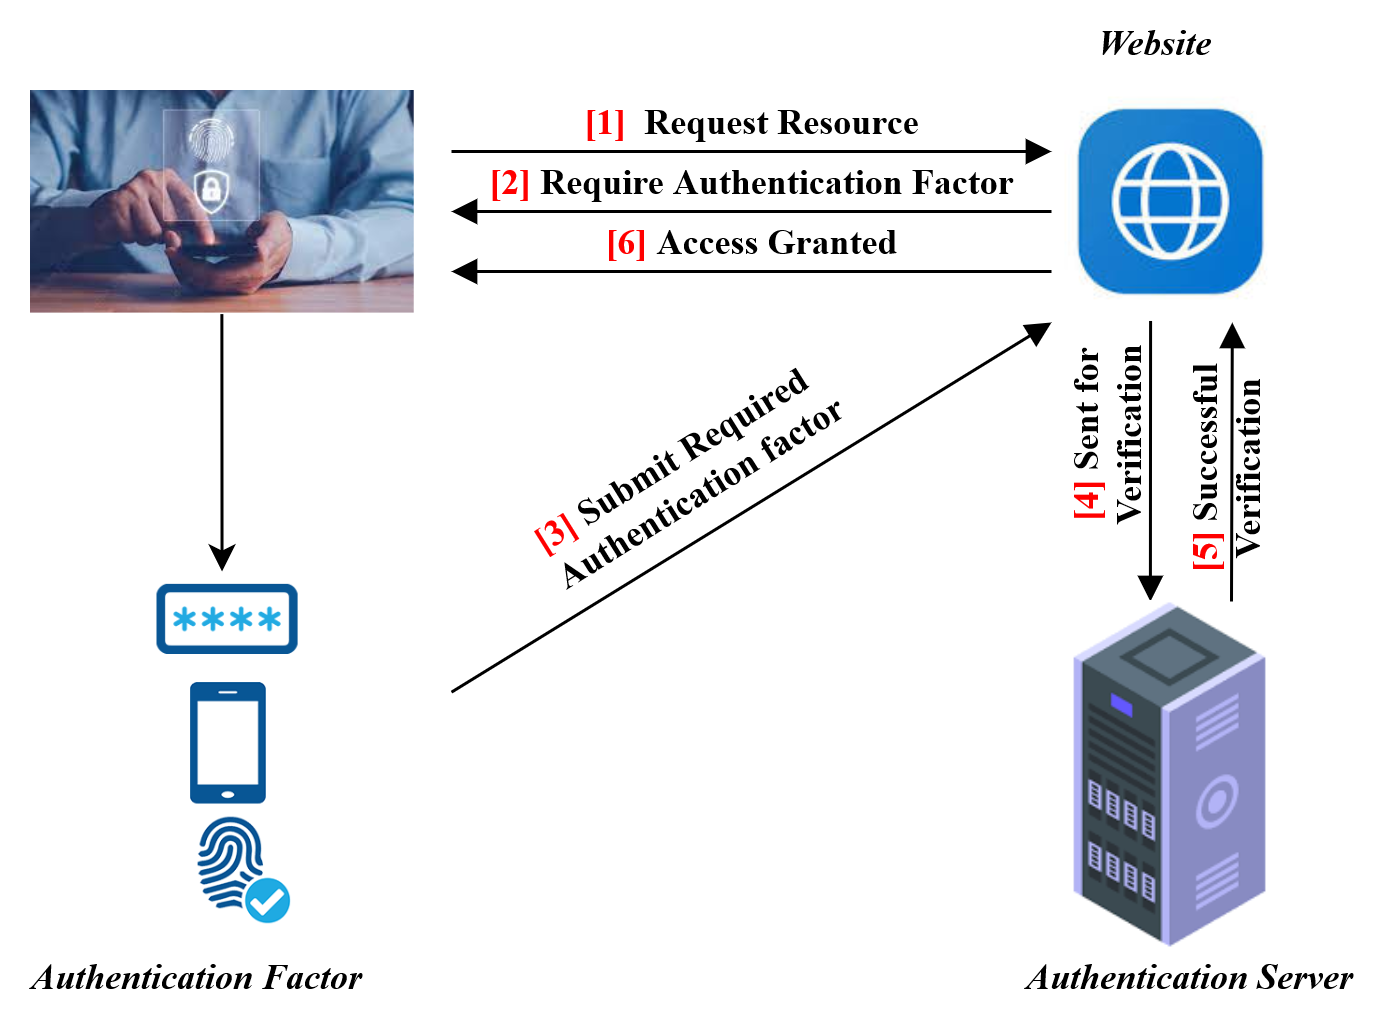
\includegraphics[width=0.75\textwidth]{Picture1_1.png}
\caption{Authentication Scenario}
\label{fig:1}
\end{figure*}
 Apart from these three factors, there can be other factors like geographic location, IP address, behaviour factors, etc. But those, as mentioned earlier, three are the most commonly categorized. 
 \par Figure \ref{fig:1} shows an authentication scenario using any of the three authentication factors. The steps followed by a user to perform authentication are described as follows:
 \begin{enumerate}
     \item User requests for a particular resource. This resource can be a website, social media account, or digital payment service.
     \item This resource access is provided only after submitting specific credentials. These credentials can be either of the three authentication factors discussed above or a combination. So, the website asks for an authentication factor.
     \item User submits required authentication factor to the website.
     \item Website sends the presented credential to the authentication server for verification.
     \item The Authentication server performs the necessary checks to complete the verification. If verification is successful, the website is given a successful verification message.
     \item Website then provides the user with access to the requested resource.
 \end{enumerate}
\subsection{Cataloguing of Authentication schemes}
Various authentication schemes have been proposed so far. In the beginning, authentication systems mainly relied on single-factor authentication schemes. The most commonly used single-factor authentication approach is username and password. But passwords are the weakest security mechanisms. The personal data of 815 million Indians exfiltrated from the ICMR’s Covid-testing database has been leaked on the dark web in October 2023 \cite{s5}. The weakness linked to using passwords as an authentication mechanism leads to the adoption of two-factor authentication (2FA) and multi-factor authentication (MFA) schemes. But people often get confused between 2FA and MFA. Although 2FA and MFA involve using more than one factor for authentication, the two have significant differences. 2FA uses two factors for authentication. For example, the password plus OTP sent through SMS or email is 2FA. At the same time, MFA consists of using two or more independent authentication factors. The two factors should be from different categories. For example, a password plus biometric sample (e.g. Iris )  is MFA, but a password in combination with OTP cannot be regarded as MFA. Velasquez, Cora and Rodreguez have found 515 single-factor and 442 multi-factor authentication techniques in their research.\cite{IEEEtran}\\
 A broad classification of various authentication schemes is shown in figure \ref{fig:2}.
 \begin{sidewaysfigure*}[!htbp]
\centering
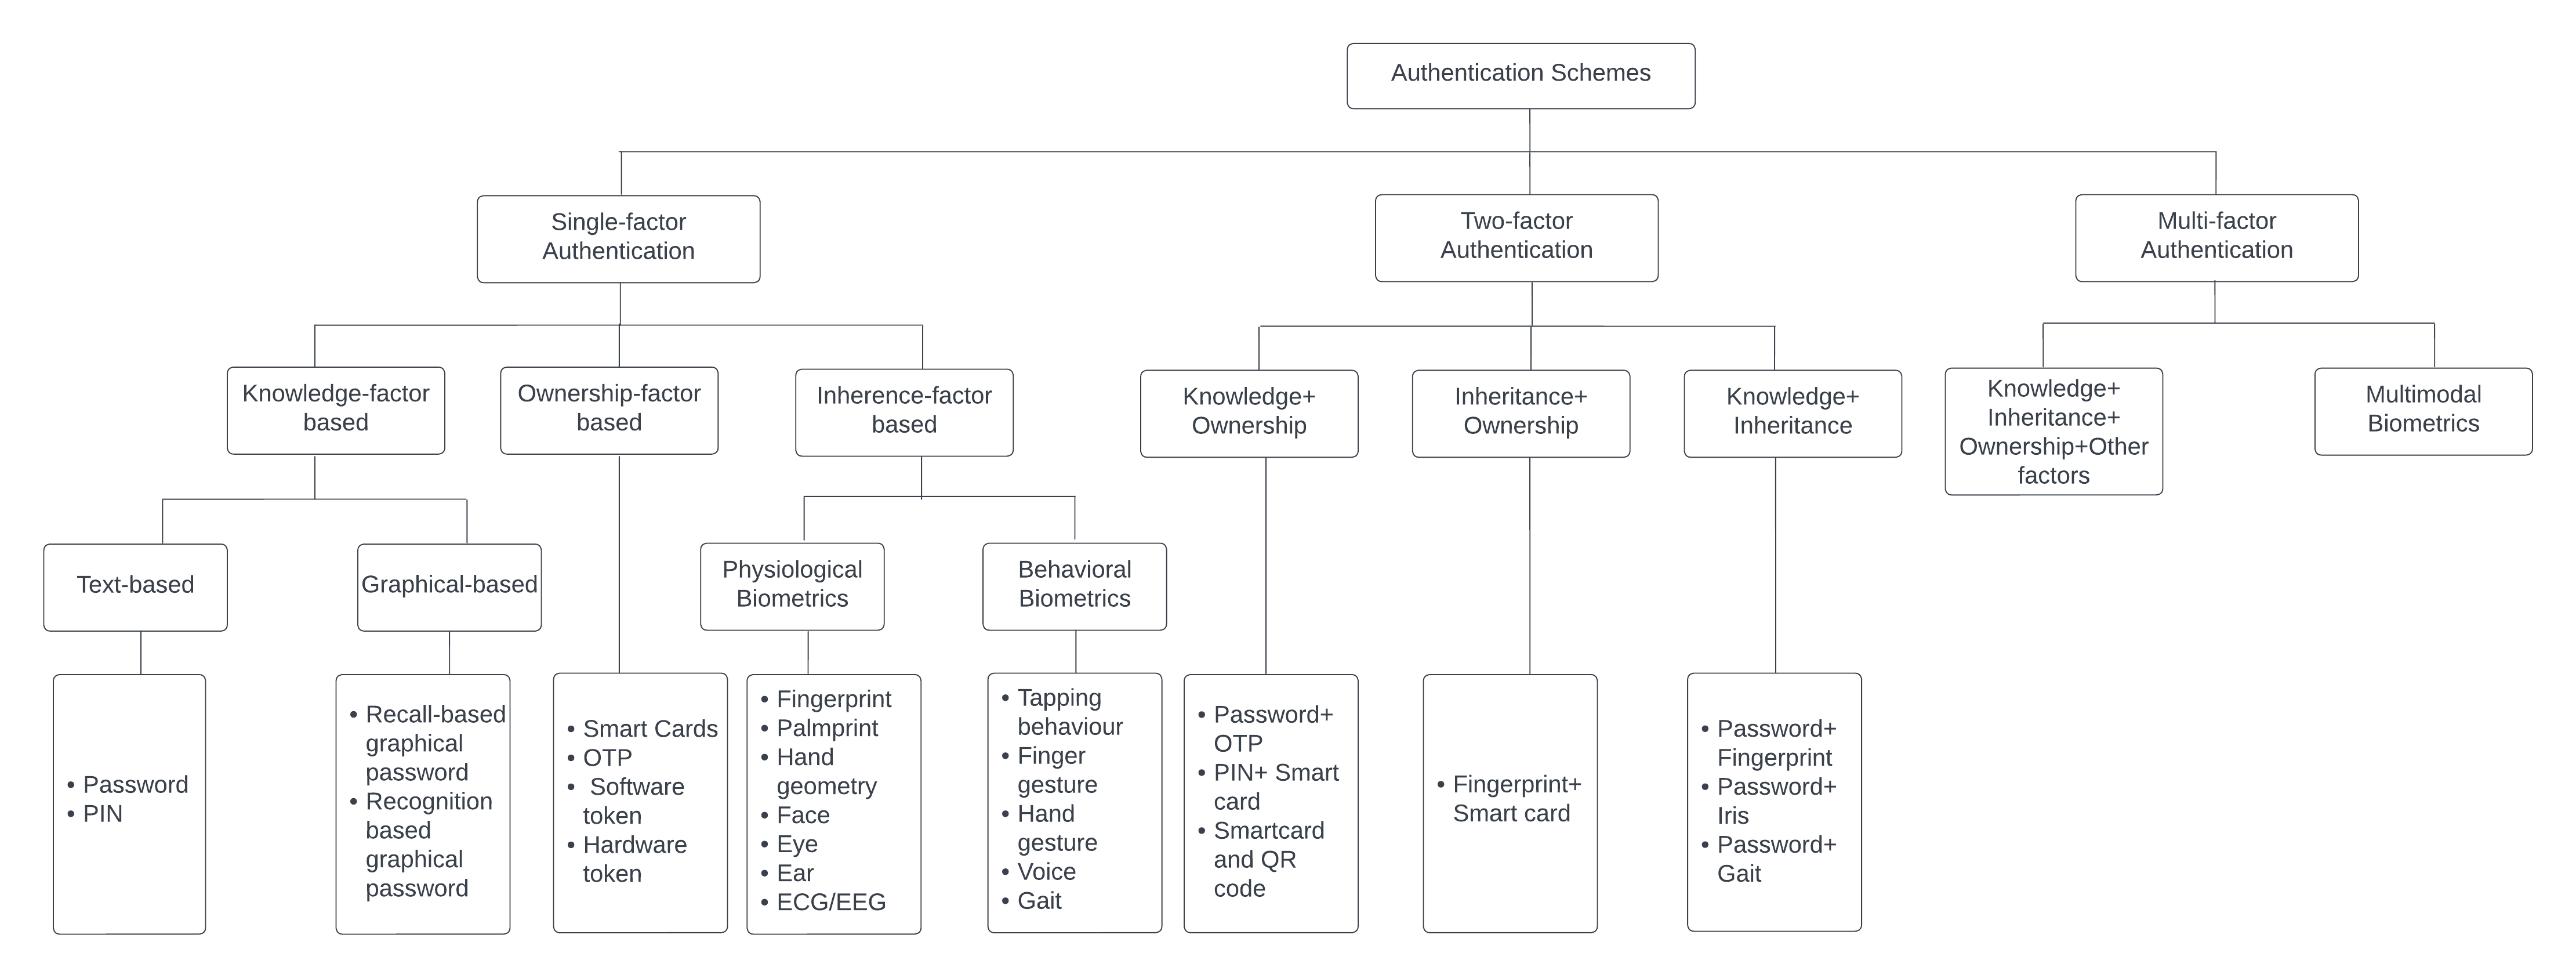
\includegraphics[width=1\textwidth]{Picture2.png}
\caption{Cataloguing of Authentication Schemes}
\label{fig:2}
\end{sidewaysfigure*}
 The schemes of authentication are mainly categorized as Single-factor authentication,two-factor authentication(2FA) and multi-factor authentication(MFA).
 \subsubsection{Single factor authentication}
      In single-factor authentication, the user uses only one metric for authentication. This metric can either be a knowledge factor (for example, passwords), a possession factor (for example, smart card) or an inherence factor (for example, fingerprint, iris scan, voice, gait, etc.). These are further divided into three types:\\
      \begin{enumerate}
          \item Knowledge-factor based\\
         This includes single-factor authentication involving only knowledge factors like passwords, PIN, etc. This is further divided into two categories based on the secret used:
          \begin{enumerate}
              \item Text-based secret\\
              This includes those secrets written in text formats like Password and PIN by using alphanumeric characters. The problem with text-based secrets is that users keep the same password for different accounts, which poses a severe security threat such that if one account is compromised, all other accounts are also at risk.
              \item Graphical-based secret\\
              Graphical-based secrets solve the problem associated with text-based secrets by selecting a set of images from the images displayed on the screen and then selecting those images at the time of authentication. It is further categorized into two types:
              \begin{enumerate}
                  \item Recognition-based Graphical password\\
                  In this authentication scheme, the user must select specific images that they have chosen at registration. One example is Passface \cite{IEEEtran61}, in which the user has to determine four face images from a database of faces as their password.
                  \item Recall-based Graphical password\\
                 In this authentication scheme, the user has to produce the drawing again that they have drawn at the time of registration. An example of this technique is Passpoint \cite{IEEEtran60}, where a user can select any location on an image to create a password. A tolerance range is calculated around each selected pixel. To authenticate, the user must click within the tolerance range of their chosen pixels, following the same order.
              \end{enumerate}
              
          \end{enumerate}
          \item Ownership-factor based\\
          This includes single-factor authentication involving only ownership factors like Smart cards, hardware tokens, mobile phones, OTP, etc.
          \item Inheritance-factor based\\
          This includes single-factor authentication involving only inherence factors like fingerprint, face, iris, retina, gait, hand geometry, etc. This is further divided into two categories:
          \begin{enumerate}
              \item Physiological Biometrics\\
              These biometrics include the physical characteristics of an individual. These characteristics are inherent to a person and cannot be changed. Examples are fingerprint, palmprint, Hand geometry, face, iris, retina, ECG, EEG, etc.
              \item Behavioral Biometrics\\
              These biometrics include human behaviour and how a person performs a particular action. These are subject to environmental changes. Examples are tapping behaviour, finger gestures, hand gestures, voice, gait, etc.
          \end{enumerate}
          \end{enumerate}
      \subsubsection{Two factor authentication}
     In two-factor authentication, the user uses two metrics for authentication. In addition to one factor, the second factor provides an extra layer of security. The two metrics can be a combination of knowledge and possession factor, knowledge and inherence factor or inherence and possession factor. Two-factor authentication (2FA) enhances security and is designed to protect the user's confidential information from unauthorized users. Passwords are unsafe means of authentication; 2FA requires an additional form of identification to prove you are who you claim to be. The two factors typically used for authentication are something you know (such as a password or PIN) and something you have (such as a mobile device or security token). There is another factor, something you are (Biometrics), which is also included to further enhance the security owing to its advantage over the other two factors. By requiring both factors, 2FA significantly increases the difficulty of someone gaining unauthorized access to your account. There are several reasons why 2FA is required. Some of these are stated below:\\
     \begin{enumerate}
         \item Passwords can be easily compromised: Passwords are a weak form of authentication because they can be easily guessed, stolen or hacked. 2FA provides extra security to protect the system even if a password has been compromised.
         \item Protection against phishing attacks: Phishing attacks are when attackers attempt to trick you into providing your login credentials or other sensitive information. With 2FA, even if an attacker can access the password, they cannot get access until they have a second factor.
         \item Compliance: Many regulations and standards require organizations to implement 2FA to protect sensitive information and prevent unauthorized access.
      \end{enumerate}
      
Generally, 2FA is an effective way to meet security needs and protect confidential data. Two factors used in 2FA can be from any of the authentication categories. \cite{IEEEtran62} proposed a 2FA that uses password and OTP. \cite{IEEEtran22} uses smart cards and QR codes as two factors in their authentication scheme. ATMs also employ 2FA by using PINs and smart cards. All these 2FA schemes discussed involve knowledge and ownership factors. Some schemes have also been proposed in the literature that involve a combination of inherence and ownership factors. \cite{IEEEtran63} proposes a scheme that uses fingerprints and smart cards for authentication. There are certain schemes in which knowledge and inheritance factors are combined to verify the identity. Examples include schemes proposed by \cite{IEEEtran64} that use password and fingerprint and by \cite{IEEEtran65} that use PIN and iris.
\subsubsection{Multi factor authentication}
      With the advancement in technology, passwords alone are insufficient to verify identity. Although 2FA adds a second factor to the conventional authentication method, there is no standard for selecting a second factor. The second factor chosen might be attack-prone and can be compromised easily. So, we need to move towards a more secure authentication mode involving two or more authentication factors with the restriction that the factors used should be independent. Multi-factor authentication is shown in figure \ref{fig:3}. In Multi-factor authentication (MFA), users need to provide multiple forms of identity to access a system or application. MFA is becoming increasingly important today, where security breaches and identity theft are more common. In multi-factor authentication(MFA), all three factors, viz. knowledge, possession and inherence, can be combined for authentication. Multiple layers of information are added to a single factor, like a password for authentication. 
The purpose of MFA is to make the authentication process difficult for illegitimate users. MFA allows users to access accounts or systems by providing at least two different forms of identity. This includes:
\begin{itemize}
\item What the user knows. e.g. Password or PIN code
\item what the user has. e.g. mobile phone or token device
\item what the user is, e.g. biometric factors such as fingerprint or facial recognition
\end{itemize}
\begin{figure}[htbp]
\centering
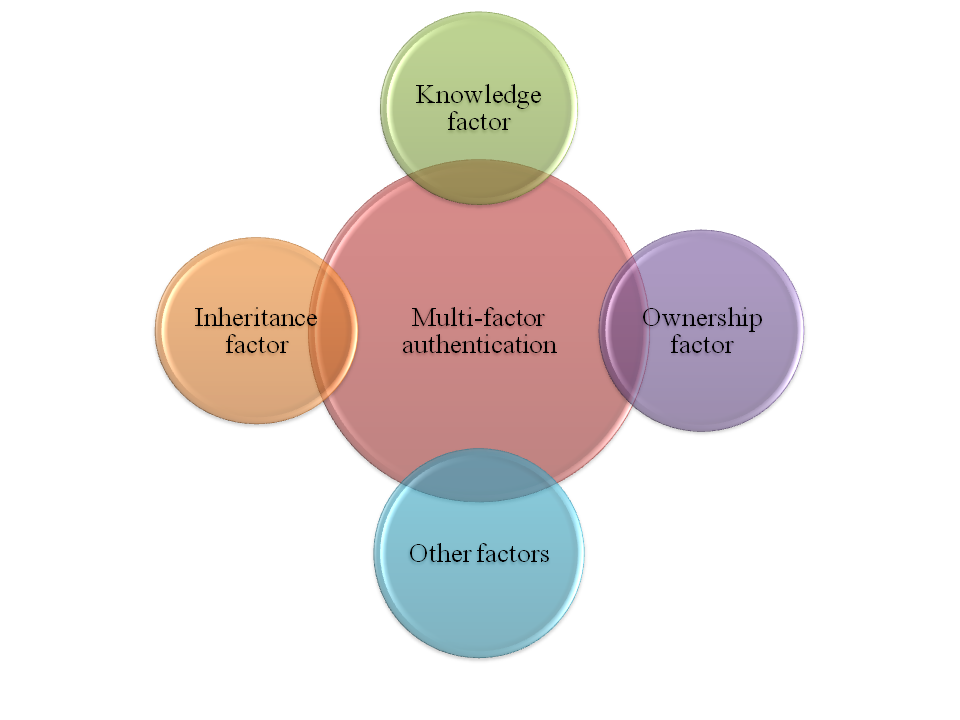
\includegraphics[width=0.5\textwidth]{Picture3.png}
\caption{Multi-factor Authentication}
\label{fig:3}
\end{figure}
MFA is commonly used in online banking, email, social media, and other applications where security is of utmost importance. It is a simple and effective way to enhance the security and protection of any system. 
      For example, the user must submit an OTP and provide their fingerprint scan in addition to the password. Various multi-factor authentication schemes have been proposed in the literature.
      \par Lee et al. \cite{IEEEtran40} introduced an authentication scheme that leverages smart card and fingerprint verification, improving security and reliability. The fingerprint verification relies on minutiae extraction and matching, while the scheme is based on ElGamal's public key cryptography using two secret keys. Scaria and Mengalingm \cite{IEEEtran51} proposed a multi-factor authentication scheme which comprises three factors - OTP, Fingerprint and noisy password. In this method, a noisy password includes a genuine password concealed within the noise, which only authorized users are aware of. Abdurrahman et al. \cite{IEEEtran30}  introduced a multi-factor authentication method called PGT, which is an acronym for pre-shared number, GPS location, and time stamp. This method is designed to boost the security of web accounts by creating a confidential hash code that incorporates the user's current GPS location and a pre-shared number.
      \subsubsection{Biometric Authentication}
      Conventional methods of authentication generally involve one or both knowledge and possession factors. However, the problems associated with these factors led to the evolution of biometric authentication.
      Biometric authentication uses physiological or behavioural traits of human beings to verify identity and authenticate to the system. This type of authentication offers certain advantages over traditional methods. This prevents imposters from attacking the system, as these traits are unique to each individual and cannot be forged. This also provides passwordless authentication, thereby lowering dependence on passwords. However, most systems using biometrics as authentication only employ single biometrics. Using a single biometric factor potentially lowers the authentication system’s accuracy rate due to poor data quality, the overlap between identities and limited resources to uniquely identify a person. Unimodal biometrics suffer from the disadvantages mentioned below-
    \begin{enumerate}
        \item Noise: The noise in sensed data can be attributed to defective or poorly maintained sensors, such as a fingerprint sensor that has accumulated dirt, resulting in deformed and noisy data. Additionally, environmental factors such as cold temperatures can affect voice recognition, while wearing glasses can alter iris recognition performance and variations in lighting conditions can impact facial recognition.
        \item Distinctiveness: Another challenge in biometric recognition is distinctiveness, which involves the significant variation of a biometric trait across individuals. Intra-class
divergences occur when a user interacts with the sensor incorrectly or exhibits an incorrect facial pose. At the same time, inter-class similarities may be present due to overlaps in
the feature sets of multiple users.
\item Non-universality: Non-universality is another issue when the biometric system cannot acquire
meaningful data from a particular group of users. For instance, scars or cuts on fingerprints may affect the accuracy of a fingerprint-based biometric system, leading to incorrect minutiae feature extraction. Faulty user-sensor interaction can also result in undesired matching results.
\item  Spoofing: Spoof attacks are another challenge wherein an imposter person attempts to spoof the biometric system using fake biometric traits or data from an authorized user. For example, by using artificial fingers or fingerprints.
    \end{enumerate}
These problems result in higher false acceptance rates (FAR) and false rejection rates (FRR). Multimodal biometrics has emerged as a solution to some of the issues in unimodal biometrics, offering benefits such as enhanced recognition accuracy, privacy, and improved biometric data
enrollment. In this, multiple biometrics features are combined for authentication and are called multimodal biometrics.
      
    \subsection{Research problem and motivation}
    Researchers are trying to find a more secure and robust authentication mechanism to combat security threats and prevent the system from cyber-attacks. Single-factor authentication cannot be a secure authentication method because the password is the main factor used for authentication, and passwords are unsafe and subject to various attacks like guessing and brute-force attacks. Passwords provide the weakest links for the attacker to access the system. MFA  and passwordless authentication is gaining popularity and becoming the current trend. In the previous subsection, the benefits of biometric authentication are discussed and how multimodal biometric authentication can be a viable solution. Multimodal biometrics, which involves more than one biometric trait, is a secure and effective authentication mode. All the schemes based on multimodal biometrics involve some problems like 
\begin{itemize}
    \item interacting with different devices to provide biometric identity
    \item The extra cost involved in purchasing devices
\end{itemize}
So, \textcolor{red}{\sout{there was no scheme which allowed parallel acquisition of biometrics}}\textcolor{blue}{existing multimodal schemes typically acquire each trait through a dedicated sensor and rarely bind acquisition to a per-session challenge; the proposed scheme instead combines parallel acquisition of biometrics from a single commodity sensor with binding of that acquisition to a fresh server-issued challenge}.

{\color{blue}
\subsection{\textcolor{blue}{Threat Model}}
We consider an adversary whose goal is to authenticate as a legitimate user to the verifier. The adversary is assumed to (i) observe and record public or previously transmitted media of the victim, including video captured in earlier sessions, (ii) mount phishing and real-time relay attacks in which a fraudulent site forwards credentials to the genuine verifier, and (iii) attempt presentation attacks by replaying a pre-recorded video of the victim. The verifier and the server-side challenge generator are assumed to be honest; the client device and the network path between the client and the verifier are untrusted. Attacks that require compromising the verifier itself, coercing the enrolled user, or synthesising a real-time deepfake that reproduces an unpredictable challenge within the session window are outside the scope of this work, as is a real-time relay that forwards the live challenge to the victim and returns the response within its validity window. Under this model, the security argument of the proposed scheme rests on two properties: the challenge is unpredictable and single-use, so a recorded response is not accepted in a later session; and the AND-based fusion rule requires every factor to be verified, so compromise of any single modality is insufficient for a successful login.
}

 \subsection{Major Contributions}\label{sec:contrib}
 The proposed scheme provides a secure and higher user acceptability multimodal biometric authentication system, unlike other multimodal biometric-based authentication systems requiring interaction with separate devices or sensors. This scheme involves parallel acquisition of biometric samples, increasing usability, security and deployability. The scheme is entirely passwordless and cost-effective due to no requirement for sensors or separate physical devices to acquire biometric samples. \textcolor{red}{\sout{The use of dynamic CAPTCHA reduces video reuse/replay attacks. No prerecorded video can be used because of the availability of this feature. Dynamic CAPTCHA also adds toward the liveliness detection of a specific user because the user will speak the captcha while recording real-time video. This scheme also prevents phishing attacks due to the presence of a captcha because the CAPTCHA is dynamic, and AND rules are implied. So, CAPTCHA validation will fail in case of a phishing attack, thereby preventing unauthorized login.}}\textcolor{blue}{The dynamic CAPTCHA acts as a per-session nonce: because the challenge is generated server-side and is unpredictable to the adversary, a previously recorded video cannot satisfy the current challenge, which mitigates video reuse and replay attacks. Since the user must utter the challenge during acquisition, the spoken CAPTCHA additionally provides a challenge--response liveness cue that is bound to the same video stream from which the face and voice evidence is derived. The same mechanism raises the cost of phishing, though its limits should be stated precisely. A phishing site that harvests a recording and replays it later fails, because the challenge it was made against has already been consumed and a fresh one is unpredictable. A real-time relay that forwards the genuine verifier's live challenge to the victim and returns the victim's fresh recording within the validity window is not prevented by this mechanism alone; defending against that case requires binding the challenge to the origin, which the present design does not do. Two further contributions concern what the verifier stores and how the factors are combined. First, the scheme retains no biometric recording: enrolment reduces the recording to encrypted templates and destroys it, so the enrolment store holds no replayable media, and the stored artefact is roughly two orders of magnitude smaller than the recording it replaces. Second, the three factors are evaluated concurrently rather than as a cascade, which both removes a timing side channel that would otherwise reveal which factor failed and reduces measured authentication latency.}
 The rest of this paper is organized as follows. The related literature survey is discussed in section 2. The working of the proposed multimodal biometric authentication system is introduced in section 3. Implementation and analysis of the proposed multimodal authentication system are demonstrated in section 4. At last, this paper is concluded by section 5.
\section{Related Work}
Marasco and Albanese \cite{IEEEtran37} suggested a multi-factor authentication approach called FingerPIN, which combines knowledge and inherence factors with a fingerprint-based personal identification number(PIN). The improved version of the FingerPIN scheme \cite{IEEEtran38} strengthens the security of this scheme and makes it more user-friendly. Li and Hwang \cite{IEEEtran32} proposed a remote user authentication scheme based on biometrics which uses smart cards and relies on biometric verification, a one-way hash function, and smart card technology. Das \cite{IEEEtran33} improved the work of Li et al. and proposed a new scheme in 2011. Das's scheme does not provide resistance against the offline password guessing attack or the privileged insider attack and does not provide user anonymity. To address the limitations in Das's scheme, Lee and Hsu \cite{IEEEtran56} introduced an alternative approach that employs extended chaotic maps.
\par D. Jagadiswary and D. Saraswady \cite{IEEEtran58} proposed a scheme that combines the RSA asymmetric cryptographic algorithm with biometric traits like fingerprints, retina scans, and finger vein patterns. Puneet Gupta et al. \cite{IEEEtran61} devised a precise authentication system that utilizes finger vein technology to elevate the quality standards of vein images and mitigate noise data during extraction. Das et al. introduced a finger-vein-based Biometric Identification System that uses a Convolutional Neural Network (CNN) \cite{IEEEtran62}. Still, it does not provide robust security for complex databases, particularly in cross-matching scenarios.
\par M. Hammad et al. \cite{r1} propose two multimodal authentication systems (sequential and parallel) and use a combination of ECG and Fingerprint. They apply Convolution Neural Network (CNN) and Q-Gaussian multi-support vector machine (QG-MSVM). Using two datasets, they attained an EER of 0.14\% and 0.10\% for the sequential systems. The parallel system achieves an EER of 0.40\% and 0.32\% for respective datasets.
 \par Kim and Hong \cite{r4} propose a multimodal biometric authentication approach using teeth image and voice as biometric features. The individual matching scores obtained from the teeth image and voice are combined using a weighted summation operation, and the fused score is used to decide the acceptance or rejection. The proposed method produces results with an EER of 2.13\%.
\par Ahamed et al. \cite{r2} propose an AI-based multimodal biometric authentication model for device-level authentication that involves ECG (Electrocardiogram) and PPG (Photoplethysmography) signals. This authentication model provides results with 99.8\% accuracy and an Equal Error Rate (EER) of 0.16.

\cite{r3} propose a  scheme that combines fingerprint, face, and iris biometrics based on matching scores. The SVM classifier, the sparse SVM classifier, and the rough set fuzzy classifier are used for fusion and classification purposes.

 

Multimodal schemes proposed so far offer less usability experience and could be more cost-effective. Because user needs to submit multiple biometric samples separately, and their acquisition requires costly hardware devices or sensors. So, we design an authentication scheme that offers parallel acquisition of biometric samples and does not require expensive hardware devices or sensors. Our scheme also provides resistance to phishing attacks.

{\color{blue}
\subsection{\textcolor{blue}{Comparison with Recent Authentication Systems (2020--2026)}}\label{sec:recent}
This work is an authentication system, so the comparison below is restricted to recent work that explicitly presents a biometric \emph{authentication} (verification) procedure. Tables~\ref{tab:recent} and~\ref{tab:recentsec} compare the proposed scheme with five such systems published between 2024 and 2026 \cite{jha2024featurefusion,aanjankumar2025smartcity,jha2025ensemble,chen2026twostep,jha2025challenge}. Work whose primary contribution is biometric recognition \cite{alharbi2023facevoice}, an audio-visual recognition and presentation-attack survey \cite{mandalapu2021avpad}, a cross-modal attack on voice authentication \cite{jiang2024foice}, or biometric template-protection methods \cite{rathgeb2023btp,zhao2023deephash} is cited as supporting security literature but is not treated as a directly comparable authentication system, because those works do not themselves deploy an end-to-end authentication decision. The comparison is not a claim that the five systems fail to authenticate; each does. It identifies what each authenticates and how, and how the present architecture differs. Cells marked \emph{NR} (not reported) denote a property the cited work does not discuss; \checkmark\ is used only where the property is explicitly supported and \xmark\ only where it is explicitly absent or placed out of scope. A security property is never inferred from a paper's title or from a related property: biometric matching is not read as liveness, encryption is not read as unlinkability, liveness is not read as replay protection, and a dynamic challenge is not read as complete relay protection.

\begin{sidewaystable*}[htbp]
\centering
\caption{\textcolor{blue}{Authentication Architecture Comparison (recent authentication systems, 2024--2026). All five prior works present an explicit authentication/verification procedure. NR = not reported by the cited work.}}
\label{tab:recent}
\renewcommand{\arraystretch}{1.3}
\scriptsize
\setlength{\tabcolsep}{3pt}
\begin{tabular}{|p{2.2cm}|c|c|p{2.0cm}|p{2.3cm}|p{2.2cm}|p{2.2cm}|p{1.7cm}|p{1.9cm}|p{2.6cm}|p{2.4cm}|}
\hline
\textbf{Work + Link} & \textbf{Year} & \textbf{Explicit Auth?} & \textbf{Modalities} & \textbf{Auth.\ Structure} & \textbf{Fusion / Decision} & \textbf{Liveness / Challenge} & \textbf{Replay Prot.} & \textbf{Phishing / MITM / Relay} & \textbf{Main Security Mechanism} & \textbf{Evaluation} \\ \hline
\href{https://doi.org/10.1063/5.0234430}{Jha et al.\ [2024]} & 2024 & Yes & Face + Speech & Simultaneous (single decision) & Feature-level fusion & Texture + synchronized-speech liveness; no dynamic challenge & NR & NR & Liveness detection (feature fusion) & Recognition accuracy \\ \hline
\href{https://doi.org/10.1038/s41598-025-29048-5}{Aanjankumar et al.\ [2025]} & 2025 & Yes & Face (single trait) & Single-modal (two-network) & Feature/architecture fusion & Anti-spoof / PAD (3D mask); no dynamic challenge & Via signatures (network) & MITM/replay via Ed25519 signatures & ElGamal + AES-256; Ed25519 signatures & Acc.\ 97.1\%; EER 3.2\% \\ \hline
\href{https://doi.org/10.1177/09287329251363424}{Jha et al.\ [2025]} & 2025 & Yes & Face + Speech & Simultaneous (single decision) & Feature-level fusion; Bi-LSTM-DCNN ensemble & Liveness via eye-blink (EAR); no dynamic challenge & NR & NR & Liveness detection (eye blink) & Acc.\ 98.2\%; EER 3.23\% \\ \hline
\href{https://arxiv.org/abs/2601.06218}{Chen et al.\ [2026]} & 2026 & Yes & Face + Voice & Sequential two-step (face then voice) & Cascade (face gates voice) & NR & NR & NR & Two-step cascade & Face acc.\ 95.1\%; voice EER 3.46\% \\ \hline
\href{https://doi.org/10.12694/scpe.v26i5.4733}{Jha et al.\ [2025], challenge-response} & 2025 & Yes & Face + Speech (spoken random word) & Challenge-response, then verify & Feature-level fusion; CNN-BiLSTM & Challenge-response liveness; random word, server-delivered, session expires on failure & \checkmark\ (counters replay video via challenge) & NR & Challenge-response liveness + PAD & Acc.\ 96.81\%; EER 3.37\%; spoof-video eval \\ \hline
\textbf{Proposed Secure User Authentication Scheme} & 2026 & Yes & Face + Voice + spoken dynamic CAPTCHA & Concurrent three-factor (parallel) & Decision-level AND ($D{=}b_f{\wedge}b_a{\wedge}b_c$); server-side & Challenge-response liveness cue (not full PAD); dynamic 5-digit CAPTCHA: server-generated, single-use, id-bound, 5-min expiry, spoken & \checkmark\ (previously recorded video/challenge) & Mitigates replay-based phishing; real-time relay \xmark\ (out of scope) & AES-256-GCM templates; HMAC-pseudonymous names; encrypted account PII with HMAC email index; keys separated by security domain (signing / template / PII) and enforced at production startup; server-signed enrolment token; server-side decision & Functional end-to-end; latency; diagnostic scores; no FAR/FRR/EER (corpus too small) \\ \hline
\end{tabular}
\end{sidewaystable*}

\begin{sidewaystable*}[htbp]
\centering
\caption{\textcolor{blue}{Security Mechanism Comparison (recent authentication systems, 2024--2026). \checkmark\ = explicitly supported; \xmark\ = explicitly absent / out of scope; NR = not reported (the work is silent). Proposed-scheme notes: liveness is a challenge-response cue, not a complete presentation-attack detector; replay protection covers a previously recorded video/challenge, not all replay; phishing mitigation covers replay-based phishing only; \emph{relay} and \emph{deepfake} are \xmark\ because the threat model of Section~\ref{sec:model} places sophisticated real-time relay and real-time challenge-reproducing deepfakes out of scope; unlinkability is claimed for the biometric template store only, not the account database; \emph{raw media retention} \xmark\ means no permanent recording is kept.}}
\label{tab:recentsec}
\renewcommand{\arraystretch}{1.35}
\scriptsize
\setlength{\tabcolsep}{3pt}
\begin{tabular}{|p{2.6cm}|c|c|c|c|c|c|c|c|c|c|c|}
\hline
\textbf{Work + Link} & \textbf{Live-ness / PAD} & \textbf{Replay Prot.} & \textbf{Dyn.\ Chall.} & \textbf{Phish / MITM} & \textbf{Relay} & \textbf{Deep-fake} & \textbf{Templ.\ Prot.} & \textbf{Encr.} & \textbf{Unlink./ Pseud.} & \textbf{Raw media ret.} & \textbf{Server dec.} \\ \hline
\href{https://doi.org/10.1063/5.0234430}{Jha et al.\ [2024]} & \checkmark & NR & NR & NR & NR & NR & NR & NR & NR & NR & NR \\ \hline
\href{https://doi.org/10.1038/s41598-025-29048-5}{Aanjankumar et al.\ [2025]} & \checkmark & \checkmark & NR & \checkmark & NR & NR & \checkmark & \checkmark & NR & NR & NR \\ \hline
\href{https://doi.org/10.1177/09287329251363424}{Jha et al.\ [2025]} & \checkmark & NR & NR & NR & NR & NR & NR & NR & NR & NR & NR \\ \hline
\href{https://arxiv.org/abs/2601.06218}{Chen et al.\ [2026]} & NR & NR & NR & NR & NR & NR & NR & NR & NR & NR & NR \\ \hline
\href{https://doi.org/10.12694/scpe.v26i5.4733}{Jha et al.\ [2025], challenge-response} & \checkmark & \checkmark & \checkmark & NR & NR & NR & NR & NR & NR & NR & \checkmark \\ \hline
\textbf{Proposed Scheme} & \checkmark & \checkmark & \checkmark & \checkmark & \xmark & \xmark & \checkmark & \checkmark & \checkmark & \xmark & \checkmark \\ \hline
\end{tabular}
\end{sidewaystable*}

\emph{Positioning.} Prior work demonstrates that multimodal biometric authentication, liveness detection, challenge-response authentication and biometric template protection have each been investigated. The proposed scheme does not claim novelty for these individual components in isolation. Its contribution is their integration into a single deployed authentication architecture combining face verification, speaker verification and a fresh spoken challenge, with concurrent factor evaluation, decision-level conjunctive fusion, template-only storage, authenticated encryption, pseudonymous template naming, enrolment binding and explicit challenge lifecycle controls. Table~\ref{tab:recentsec} shows that no single prior authentication system in the comparison combines a session-bound spoken challenge with protected, pseudonymous template storage and a server-side conjunctive decision; the closest, a challenge-response multimodal system \cite{jha2025challenge}, shares the spoken challenge and liveness properties but does not report template protection, encryption, pseudonymous storage or enrolment binding, and fuses at the feature level rather than combining independent per-factor decisions.

\noindent The closest differences are as follows.
\begin{enumerate}
\item Compared with Jha et al.\ [2024] \cite{jha2024featurefusion}: face + speech with texture/speech liveness, fused at the feature level; the present scheme adds a server-generated dynamic spoken challenge and a template-storage and enrolment-security architecture, and combines independent per-factor decisions rather than fused features.
\item Compared with Aanjankumar et al.\ [2025] \cite{aanjankumar2025smartcity}: a single-trait facial authentication system with strong cryptographic storage and signature-based transport protection; the present scheme is multimodal (face + voice + spoken challenge) and adds a challenge-response liveness cue and pseudonymous template naming, while not claiming the signature-based MITM property that work reports.
\item Compared with Jha et al.\ [2025] \cite{jha2025ensemble}: feature-level multimodal face/speech fusion with eye-blink liveness; the present scheme uses independent factor decisions combined by an AND rule at the decision level, and adds a session-bound challenge and protected storage.
\item Compared with Chen et al.\ [2026] \cite{chen2026twostep}: a sequential two-step face-then-voice cascade; the present scheme evaluates face, voice and the spoken CAPTCHA concurrently and combines them conjunctively, which also removes the timing side channel of a cascade and returns an identical response whichever factor fails.
\item Compared with the challenge-response multimodal system Jha et al.\ [2025] \cite{jha2025challenge}: both use a random spoken challenge for liveness; the present scheme's challenge is server-generated, single-use, identifier-bound and expiring, is integrated with face and speaker verification under decision-level AND fusion, and is paired with AES-256-GCM encrypted, HMAC-pseudonymously-named template-only storage and token-bound enrolment, none of which that work reports.
\end{enumerate}

\emph{Evaluation scope.} Among the compared systems, recognition-oriented accuracy, EER and related rates are reported by \cite{jha2024featurefusion,aanjankumar2025smartcity,jha2025ensemble,chen2026twostep,jha2025challenge}, and \cite{jha2025challenge} additionally reports a spoof-video evaluation. The present work does not report FAR, FRR or EER: its current corpus is too small for a meaningful error-rate claim (Section~\ref{sec:limits}). It instead reports diagnostic matcher score separation (Table~\ref{tab:scores}), functional end-to-end authentication behaviour, and processing latency (Section~\ref{sec:perf}), where concurrent evaluation overlaps the biometric and challenge branches and reduces mean end-to-end latency from 15{,}320\,ms (cascaded) to 13{,}293\,ms (concurrent), a reduction of approximately 2{,}027\,ms ($\approx$1.15$\times$). Accuracy figures across these systems are measured on different datasets and protocols and are therefore not directly comparable, and no such cross-system accuracy claim is made here. Consistent with the threat model of Section~\ref{sec:model}, the scheme does not claim to defeat sophisticated real-time relay attacks or real-time deepfakes that reproduce an unpredictable challenge within the validity window, and the spoken challenge is a liveness cue rather than a complete presentation-attack detector.
}

\section{The Proposed Scheme}
The proposed scheme relates to multimodal biometric systems. Notably, it specifies a more secure and user-friendly biometric authentication system. This scheme provides a multimodal biometric authentication system that combines face and voice. In addition to biometrics, a dynamic CAPTCHA was also present. Each biometric feature proposed in the scheme and the CAPTCHA was extracted from the real-time recorded video. The three credentials used in the scheme are matched according to the AND logic rules. This ensures that successful authentication is achieved only when all the credentials are compared positively.
\textcolor{red}{\sout{The present invention also provides an authentication system that involves the parallel acquisition of biometric features.}}\textcolor{blue}{The scheme therefore realises parallel acquisition of biometric features: a single video stream is the common source from which all factors are derived, so the acquisition cost is independent of the number of modalities.}
\\

{\color{blue}
\subsection{\textcolor{blue}{System Model and Decision Rule}}\label{sec:model}
Let $V_r$ and $V_l$ denote the videos acquired during registration and login respectively, and let $C$ denote the CAPTCHA string issued by the server for the current session. Three decisions are derived from the single login stream:
\begin{itemize}
    \item a face decision obtained by scoring the login recording's per-frame face embeddings against the enrolled face embedding at a threshold $\tau_f$;
    \item a voice decision obtained by scoring the login speaker embedding against the enrolled speaker embedding at a threshold $\tau_a$;
    \item a challenge decision obtained by transcribing the login audio and comparing the transcript with $C$.
\end{itemize}
Both biometric factors are scored by \emph{similarity} rather than distance: each modality is reduced to an L2-normalized embedding, so the inner product of two embeddings is their cosine similarity and a factor is accepted when that similarity reaches its threshold. Let $e_r^{f}$ denote the enrolled face embedding and $\{e_{l,i}^{f}\}_{i=1}^{n}$ the per-frame embeddings of the login recording, and let $e_r^{a}$, $e_l^{a}$ denote the enrolled and login speaker embeddings. Writing $T(\cdot)$ for the speech-to-text transform and $\mathcal{N}(\cdot)$ for the CAPTCHA normalization map, the factor decisions are
\begin{equation}
b_f = \mathbb{I}\Big[\operatorname{median}_{i}\big\langle e_r^{f},\, e_{l,i}^{f}\big\rangle \;\geq\; \tau_f\Big],
\label{eq:face}
\end{equation}
\begin{equation}
b_a = \mathbb{I}\Big[\big\langle e_r^{a},\, e_l^{a}\big\rangle \;\geq\; \tau_a\Big],
\label{eq:voice}
\end{equation}
\begin{equation}
b_c = \mathbb{I}\Big[\exists\, t \in T(A_l): \mathcal{N}(t) = \mathcal{N}(C)\Big],
\label{eq:captcha}
\end{equation}
where $\mathbb{I}[\cdot]$ is the indicator function. The face score is the \emph{median} of the per-frame similarities rather than the mean, so that a minority of degraded frames (motion blur, partial pose, transient occlusion) cannot move the verdict. The challenge decision accepts if \emph{any} transcription hypothesis matches after normalization, because the speech-to-text stage returns a ranked list of alternatives and the correct reading of a spoken digit string is frequently not the top-ranked one.
Fusion is performed at the decision level under a conjunctive rule,
\begin{equation}
D = b_f \wedge b_a \wedge b_c ,
\label{eq:fusion}
\end{equation}
and access is granted only when $D = 1$. A conjunctive rule is chosen deliberately: it lowers the false acceptance rate at the cost of a higher false rejection rate, which is the appropriate operating point for an authentication decision, and it guarantees that the compromise of any single modality cannot by itself produce a positive decision.

An important consequence concerns \emph{when} the three decisions are computed. A conjunction may be evaluated lazily, aborting at the first negative factor, and this is what a cascaded formulation implies. The scheme deliberately does not do so: all three factors are evaluated concurrently and combined only once every verdict is available. Two properties motivate this. First, the response latency of a rejected attempt no longer depends on which factor failed, removing a timing side channel that would otherwise let an adversary probe the factors independently and reduce a conjunctive decision to three separate sub-problems. Second, the failing factor is never disclosed to the client---the rejection response is identical in every case, and the per-factor outcome is written only to the server log. Concurrent evaluation additionally overlaps the challenge branch with the biometric branch, which is the source of the latency reduction reported in Section~IV.

\begin{figure}[!htbp]
\centering
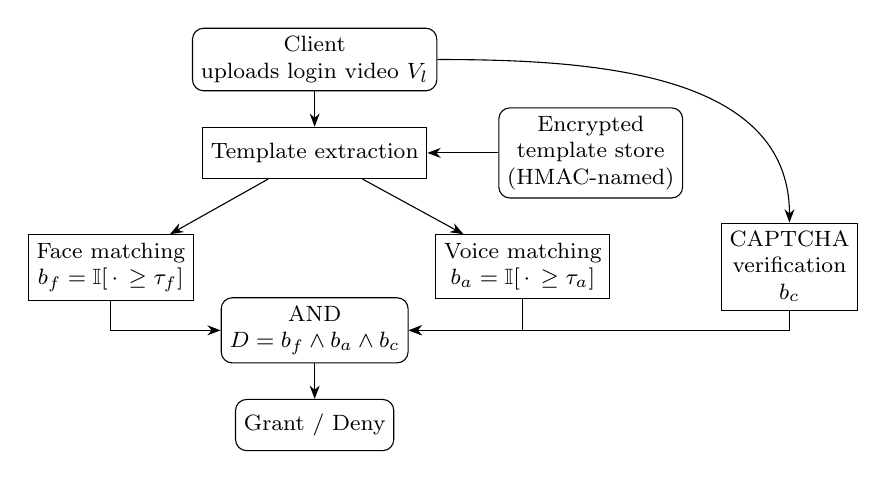
\begin{tikzpicture}[font=\footnotesize, >={Stealth[]},
  box/.style={draw, rounded corners, align=center, inner sep=3pt, minimum height=6.5mm},
  op/.style={draw, align=center, inner sep=3pt, minimum height=6.5mm},
  node distance=4.5mm and 7mm]
\node[box] (client) {Client\\uploads login video $V_l$};
\node[op, below=of client] (extract) {Template extraction};
\node[op, below left=7mm and 1mm of extract] (face) {Face matching\\$b_f=\mathbb{I}[\,\cdot\,\ge\tau_f]$};
\node[op, below right=7mm and 1mm of extract] (voice) {Voice matching\\$b_a=\mathbb{I}[\,\cdot\,\ge\tau_a]$};
\node[op, right=14mm of voice] (cap) {CAPTCHA\\verification\\$b_c$};
\node[box, below=15mm of extract] (and) {AND\\$D=b_f\wedge b_a\wedge b_c$};
\node[box, below=of and] (out) {Grant / Deny};
\node[box, right=9mm of extract] (store) {Encrypted\\template store\\(HMAC-named)};
% biometric branch
\draw[->] (client)--(extract);
\draw[->] (extract)--(face);
\draw[->] (extract)--(voice);
\draw[->] (store)--(extract);
% challenge branch runs concurrently, from the same recording
\draw[->] (client.east) to[out=0,in=90] (cap.north);
% fusion
\draw[->] (face) |- (and);
\draw[->] (voice) |- (and);
\draw[->] (cap) |- (and);
\draw[->] (and)--(out);
\end{tikzpicture}
\caption{\textcolor{blue}{Deployed concurrent authentication architecture. The uploaded login video feeds two independent branches evaluated in parallel: a biometric branch that reduces the recording to one login template and scores face and voice against the enrolled encrypted template, and a challenge branch that transcribes the audio and verifies it against the issued CAPTCHA. The enrolled reference is an AES-256-GCM encrypted, pseudonymously named template, never a stored recording. The three verdicts are combined by the conjunctive rule of equation~(\ref{eq:fusion}); access is granted only when all three pass, and the response is identical whichever factor fails.}}
\label{fig:concurrent}
\end{figure}

\subsection{\textcolor{blue}{Feature Representations}}\label{sec:features}
The scheme is agnostic to the specific matchers, but the representations it instantiates determine whether the factors are genuinely discriminative, and two of the representations originally adopted were found not to be.

\emph{Face.} The face factor was initially specified as a perceptual hash (pHash) of whole frames compared by Hamming distance. A perceptual hash summarises an entire frame---background, illumination and pose along with the subject---so it measures scene similarity rather than identity. On our own recordings the genuine pair \texttt{123} vs \texttt{123\_l} scored a Hamming distance of 26.0 against the specified acceptance threshold of 25, i.e.\ a genuine user was falsely rejected, while impostor pairs scored 30.0 and 32.0; the genuine and impostor populations are therefore not separated by a usable margin. The face factor accordingly uses face detection followed by a 512-dimensional deep embedding trained with an additive angular margin objective \cite{arcface}, compared by cosine similarity as in equation~(\ref{eq:face}). On the same four pairs the embedding scores 0.7265 and 0.6194 for genuine pairs and 0.2247 and 0.1838 for impostor pairs against a threshold $\tau_f = 0.35$, separating both populations on this data. These are four pairs drawn from a handful of recordings, not an accuracy evaluation: they establish that the replaced statistic failed on cases where the embedding succeeds, and they are reported for that diagnostic purpose only. No false-acceptance or false-rejection rate is claimed from them. Twelve frames are sampled uniformly across each recording; the enrolled reference is the L2-normalized mean of the per-frame embeddings.

\emph{Voice.} The voice factor was initially specified as a 13-coefficient MFCC matrix compared by mean pairwise Euclidean distance. Measured across the four enrolled templates then available, belonging to two distinct speakers, this statistic did not separate speakers at all: genuine same-speaker pairs scored 172.8--178.8 while impostor pairs scored 153.7--193.0, so the impostor range strictly contains the genuine range and the closest pair of all was an impostor pair. No threshold on this statistic separates speakers on this data, and the factor was observed accepting a different speaker in practice. The cause is structural rather than a matter of calibration---the distance is dominated by frame log-energy, whose zeroth coefficient is an order of magnitude larger than the remaining coefficients, and by the dispersion of the two frame clouds, i.e.\ by loudness and recording conditions. Text-independent speaker verification instead requires a discriminative learned embedding, so the voice factor uses a 192-dimensional ECAPA-TDNN speaker embedding \cite{ecapa} scored by cosine similarity as in equation~(\ref{eq:voice}), which is structurally the same decision the face factor makes. The operating threshold $\tau_a = 0.30$ is taken from a measured cosine distribution rather than assumed: over the labelled window pairs available, real cross-speaker pairs reached at most 0.256 while genuine same-speaker pairs floored at 0.345, and 0.30 lies in that gap. That distribution rests on two speakers, so it fixes a defensible operating point on the available data; it is not an equal-error-rate calibration and no error rate is claimed for it.

\subsection{\textcolor{blue}{Security Mechanisms}}\label{sec:security}
Seven mechanisms carry the security argument of Section~\ref{sec:contrib}.

\emph{Template-only storage.} No recording of any user is retained. The registration video is reduced to the two embeddings above and destroyed; only the embeddings are stored. This matters because an embedding is not a playable recording of the subject's face and voice, so a breach of the enrolment store does not yield reusable biometric media. The stored artefact is also two orders of magnitude smaller than the recording it replaces.

\emph{Encryption at rest with integrity.} Templates are sealed under AES-256-GCM \textcolor{blue}{using the dedicated template key $k_{\text{bio}}$ of the key-separation mechanism below}. The authenticated-encryption tag doubles as an integrity check: a template modified on disk fails authentication during decryption, and the scheme fails closed by rejecting the login rather than proceeding with unverified data. The login recording, which must persist briefly because two independent branches consume it, is encrypted under the same envelope \textcolor{blue}{and the same key} and deleted once the attempt resolves, whatever its outcome.

\textcolor{blue}{\emph{Key separation by security domain.} The scheme keeps three cryptographic secrets, and no operation ever borrows one domain's secret for another's purpose:}

\textcolor{blue}{\begin{itemize}[leftmargin=*,topsep=2pt,itemsep=1pt]
\item $k_{\text{sig}}$ signs session and enrolment tokens, and is used for nothing else. It authenticates statements; it encrypts no store.
\item $k_{\text{bio}}$ seals the biometric templates and the transient login recording under AES-256-GCM, and keys the pseudonymous template names $\mathrm{HMAC}(k_{\text{bio}},\cdot)$ of the next mechanism.
\item $k_{\text{pii}}$ seals the account record's contact fields under AES-256-GCM and keys the email index $\mathrm{HMAC}(k_{\text{pii}},\cdot)$ used for duplicate detection.
\end{itemize}}

\textcolor{blue}{The separation bounds what a single disclosure costs. An adversary holding $k_{\text{sig}}$ can forge tokens but cannot read a template or a contact field; one holding $k_{\text{bio}}$ can decrypt templates and re-derive their storage names but learns nothing about addresses or telephone numbers; one holding $k_{\text{pii}}$ obtains the contact details but no biometric reference and no ability to mint a token. Deriving all three from one secret---or, in the common shortcut, deriving the storage keys from the token-signing secret---would make each of those compromises the others as well, so the separation is enforced rather than merely recommended: a deployment configured for production refuses to start unless all three secrets are supplied explicitly and each is at least $32$ characters, with $k_{\text{bio}}$ and $k_{\text{pii}}$ additionally required to differ from one another and from $k_{\text{sig}}$. The signing key is subject to the same requirement in its own right, and for a reason that does not involve encryption at all: its development fallback is a constant that appears in the published source, so a deployment running on it would let anyone forge a session token---bypassing authentication outright---or an enrolment token, which is precisely the capability the enrolment-binding mechanism below exists to withhold. A production configuration that supplies that placeholder value, or a short one, is rejected exactly as a missing storage key is. The check runs before the service accepts any request and before any maintenance task can touch the stores, so a misconfigured deployment fails visibly at startup instead of serving traffic while protecting its data with a secret intended for a different purpose. A development checkout with no keys configured falls back to derived values so that a fresh clone runs; that fallback is a convenience for development only, is announced on startup, and is exactly what the production check refuses. What key separation does \emph{not} do should be equally clear: it bounds the blast radius of a key disclosure, and it neither prevents a database compromise nor, on its own, prevents account takeover---the mechanisms below address that.}

\emph{Pseudonymous storage (unlinkability).} Confidentiality and integrity protect a template's \emph{contents}, but they say nothing about what its \emph{name} discloses. If a stored template is named after the account it belongs to, then a compromise of the storage directory alone---without the database and without the encryption key---reveals the entire enrolled membership by name and yields one labelled biometric template per person, each reusable for cross-system correlation. This is the unlinkability concern of ISO/IEC~24745. Each template is therefore stored under a name that is a keyed hash of the identifier, $\mathrm{HMAC}(k_{\text{bio}},\text{id})$ under the same template key $k_{\text{bio}}$ that protects the templates, rather than under the identifier itself. A keyed hash rather than a plain one is deliberate: identifiers are low-entropy and would fall to a dictionary against an unkeyed digest, whereas an adversary who lacks $k_{\text{bio}}$ cannot map a stored name back to an identity, and one who possesses $k_{\text{bio}}$ can already decrypt the templates, so no additional linkage is conceded. \textcolor{blue}{Binding the name to the same key as the contents is deliberate in the other direction too: the naming key and the sealing key share a lifecycle, so a change of $k_{\text{bio}}$ invalidates the names and the decryptability of the templates together rather than leaving one valid and the other stale. That coupling is a consistency property, not a rotation capability---see the operational limitation stated in Section~\ref{sec:limits}.} The mapping is deterministic, so verification re-derives the name at login without any stored lookup table, and no plaintext identifier is written to the template store.

\textcolor{blue}{\emph{Scope of the unlinkability property.} This property applies to the biometric template store and should be read accordingly, including the \textit{Unlinkable} rating in Table~\ref{tab:2}. It does not extend to the account database, which is a separate store. Authentication necessarily requires an account record, and that record holds the account information supplied at registration---a unique username and email, and optionally profile fields such as name, mobile number and address. \textcolor{blue}{Of these, only the username is stored in the clear, and deliberately so: it is the lookup key queried on every login, it is submitted by the client on every request, and sealing it would impose a blind index on the hot authentication path while concealing nothing that the client does not already transmit. Every other field---email address, first and last name, mobile number, postal address and the optional avatar---is sealed under AES-256-GCM with the account key $k_{\text{pii}}$ before it is written, and opened when the profile is served. The property this provides should be stated exactly: it is confidentiality of the account record \emph{at rest}, so that a compromise of the database itself---a dump, a stolen backup, an exposed instance---yields ciphertext for every contact field. It is not an access-control property of the running service, because the prototype's profile endpoint is not authenticated and will open a record for any caller that names the identifier; adding that control is a deployment measure independent of the encryption described here. The key is the account domain's own, distinct from the template key $k_{\text{bio}}$ and from the signing key $k_{\text{sig}}$, so a disclosure confined to one domain does not extend to the others. The email address additionally carries a keyed-hash index, $\mathrm{HMAC}(k_{\text{pii}}, \mathcal{N}_e(\text{address}))$ over the case- and whitespace-normalized address, which preserves the equality test that duplicate-registration checking needs without the server ever comparing---or being able to read---a stored address. Ciphertext cannot serve that purpose itself, because the random initialisation vector makes two records holding the same address differ byte for byte; the index is keyed rather than a plain digest because addresses are guessable and an unkeyed digest would fall to a dictionary. The index is never returned to the client, since it is a stable handle for the address it stands in for.} The two stores are decoupled: the account database contains no template and no template file name, while the template store contains no plaintext identifier, so the templates are pseudonymously identified and stored separately from the account information. A compromise limited to the template directory therefore discloses neither identities nor a mapping from a stored template to one, which is the property claimed; a compromise of the account database discloses the enrolled usernames\textcolor{blue}{, but neither the contact details, which are ciphertext under a separate key, nor any biometric template}. Unlinkability is thus a property of the biometric template store, not of the account database\textcolor{blue}{: the account database is confidentiality-protected but not unlinkable, since its usernames remain readable, and making them unlinkable too would require a blind index on the login lookup path and would not conceal the identifier the client transmits on every attempt in any case. What the account encryption does buy is that the personal data attached to an identity---address, telephone number, email---no longer follows from a database dump, so the residual disclosure is the membership list rather than the contact list. Minimising the fields collected remains an orthogonal measure, and neither affects the biometric protections described above}.}

\emph{Enrolment binding.} The identity being enrolled is established by a short-lived server-signed enrolment token issued once, at account creation, and never by client-supplied data such as a filename. \textcolor{blue}{The deployed validity period is ten minutes: long enough to re-record and retry a failed upload, short enough that a leaked token is not a standing licence to re-enrol the account.} This closes an account-takeover path: if the enrolled identity is read from the uploaded filename, any unauthenticated client can replace another user's stored template with its own biometrics and then authenticate as that user. Because account creation rejects any identifier that is already \emph{enrolled}, a token can never be minted against an existing enrolment, and the enrolment endpoint independently refuses an upload for an identifier that already holds a template, so a stored template is never replaced---not even by the holder of a valid token. A session token is explicitly not accepted for enrolment, so a stolen session cannot re-key an account. \textcolor{blue}{The qualifier \emph{enrolled} is deliberate. Registration spans two requests, so it can stop between them and leave an account that holds no template. Such an account is inert---it cannot authenticate, because there is nothing to match against---but it would otherwise hold its identifier permanently, since its enrolment token expires and no second one can be issued. A failed extraction therefore rolls the account back, an identifier held by an account with no template is released to a later registration, and an enrolment is refused if the account it names no longer exists. Releasing an unenrolled identifier surrenders no biometric reference, because none was ever bound to it; releasing an enrolled one would be the takeover this mechanism exists to prevent, and is what the template check above forbids. \textcolor{blue}{One consequence of releasing an identifier should be stated precisely, because it follows from what the deployed token actually carries. The token binds the identifier and the purpose, but no account instance, and the enrolment endpoint accordingly locates the account by identifier alone. An identifier released while a previously issued token for it is still inside its ten-minute window can therefore be enrolled, by the holder of that earlier token, onto the account that subsequently claimed the same identifier. Binding the token to the account instance---by carrying an account reference in the token and requiring it to match---would remove this, and is not implemented in the prototype described here.}}

\emph{Challenge handling.} The challenge is generated server-side and only its rendered image is transmitted; the expected string never reaches the client, since a client that knows the expected text can satisfy the challenge without a live utterance. Each challenge is bound to one identifier, is consumed on the first verification attempt whether or not that attempt succeeds, and expires after a fixed window of five minutes. \textcolor{blue}{A login recording is accepted for upload only while an issued, unexpired challenge exists for that identifier, so a recording cannot be submitted outside a live login attempt.} The challenge alphabet is restricted to five decimal digits. This is a deliberate consequence of the recognition stage rather than a security choice: transcription of arbitrary letter strings proved unreliable, whereas digit sequences transcribe dependably, and the comparison of equation~(\ref{eq:captcha}) normalizes spelled-out number words to numerals before matching so that a correct utterance is not rejected for orthographic reasons. The reduced alphabet lowers the entropy of a single challenge, which is acceptable only because the challenge is not a standalone credential: it is conjoined with two biometric factors under equation~(\ref{eq:fusion}), and guessing it confers nothing without also passing them.

\emph{Input validation.} Every identifier that reaches a filesystem path or a subprocess argument is validated against a restrictive character class at account creation, at enrolment and at login, and the uploaded filename is pattern-checked rather than trusted. Without this, an identifier containing path separators would escape the intended storage directory, and the enrolled identity is in any case taken from the signed token rather than the filename.
}

The proposed authentication scheme's registration phase considers Email address and unique username. After this, the user records the real-time video while speaking the dynamic CAPTCHA. \textcolor{blue}{This recording is reduced to the biometric templates defined in Section~\ref{sec:features}, which are encrypted and stored; the recording itself is discarded and is never written to persistent storage.}
The proposed authentication system uses biometric features of face and voice. The user is required to capture a real-time video. However, while recording the video, the user must speak the dynamic CAPTCHA displayed on the screen. From this real-time recorded video, face, voice and CAPTCHA are extracted. \textcolor{blue}{The corresponding reference is not a stored recording but the encrypted template enrolled for that identifier, which was derived once at registration and retained in place of the video. Matching therefore compares the login embeddings against the enrolled embeddings, never against a second recording.} Also, the voice/audio is converted to text and matched with the dynamic CAPTCHA text displayed on the screen. All these matching results are then applied AND logic, which ensures positive authentication only if all the results are positive. These results are combined to decide whether the authentication is successful and give the final decision. Dynamic CAPTCHA reduces video reuse/replay attacks and adds to the liveliness detection of a specific user.

 Initially, we start with entering a unique username that helps in user identification and then a real-time video capturing field and dynamic CAPTCHA is displayed. The individual trying to authenticate themself records real-time video while speaking dynamic CAPTCHA, displayed on the screen. From this recorded video, frames are extracted. Also, audio is extracted from this recorded video. \textcolor{blue}{The per-frame embeddings computed from these frames are scored against the enrolled face embedding stored for that identifier.}
\textcolor{blue}{Similarly, the speaker embedding computed from the login audio is scored against the enrolled speaker embedding to decide whether the person speaking is the enrolled user. No registration audio exists on the server to be re-extracted.} Also, the extracted audio is converted to text matched with the CAPTCHA displayed for CAPTCHA validation checking. After matching frames and audio is complete, the matching score is checked to see if it is above a certain threshold and matching is successful. Then, all these results are subjected to AND logic, which gives positive results only if all validations and matching are positive. The user is granted access to resources if the result is positive. Otherwise, access is not granted.

There are three phases involved in this authentication scheme - 
\begin{itemize}
    \item Registration Phase
    \item Login Phase
    \item Authentication phase
\end{itemize}
\subsection{Registration Phase}
\begin{figure*}[!htbp]
\centering
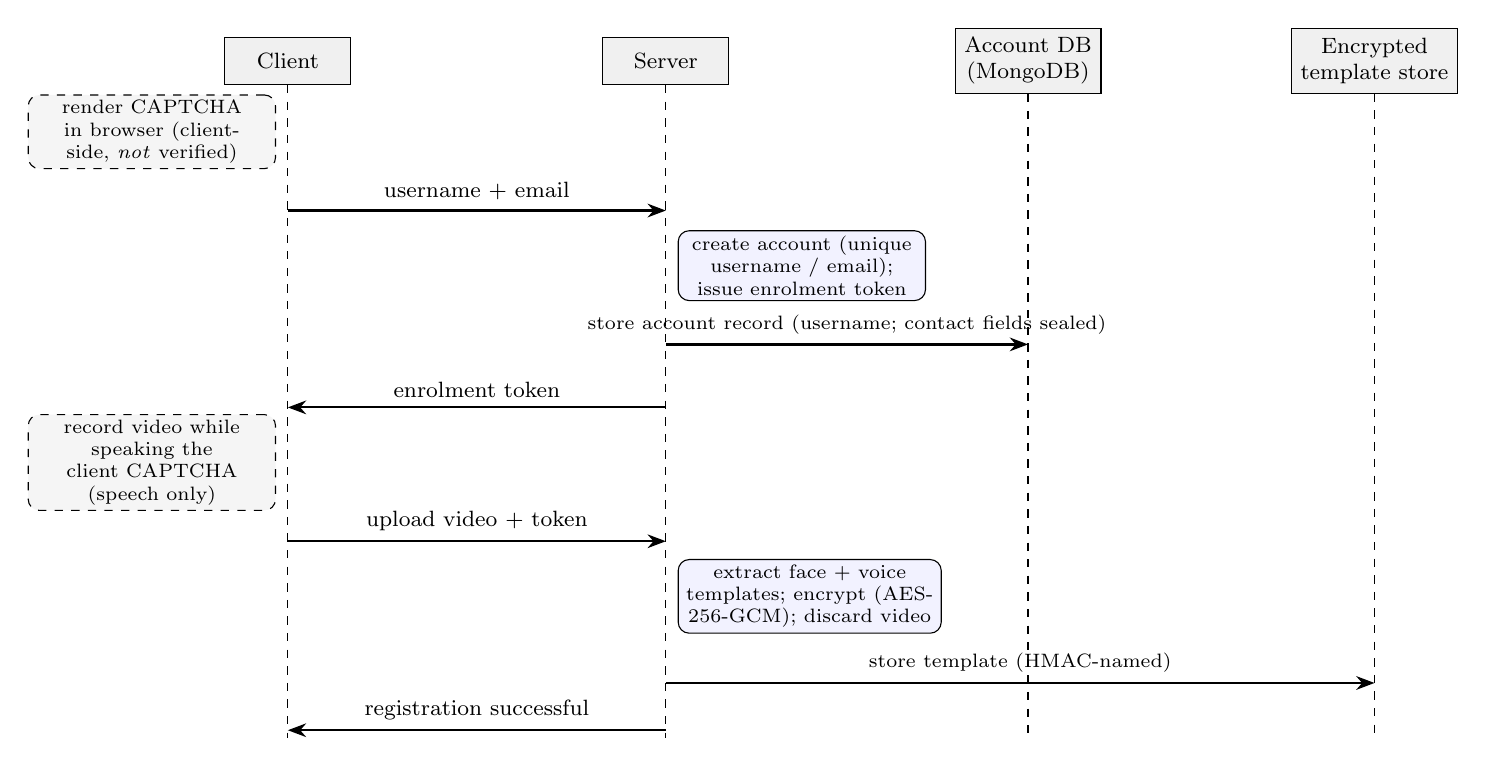
\begin{tikzpicture}[font=\footnotesize, >={Stealth[]},
  hdr/.style={draw, fill=gray!12, minimum width=16mm, minimum height=6mm, align=center},
  msg/.style={->, thick},
  note/.style={draw, fill=blue!5, rounded corners, align=center, inner sep=2pt, font=\scriptsize},
  cnote/.style={draw, dashed, fill=gray!8, rounded corners, align=center, inner sep=2pt, font=\scriptsize}]
\node[hdr] (C) at (0,0) {Client};
\node[hdr] (S) at (4.8,0) {Server};
\node[hdr] (M) at (9.4,0) {Account DB\\(MongoDB)};
\node[hdr] (T) at (13.8,0) {Encrypted\\template store};
\draw[dashed] (C.south) -- (0,-8.6);
\draw[dashed] (S.south) -- (4.8,-8.6);
\draw[dashed] (M.south) -- (9.4,-8.6);
\draw[dashed] (T.south) -- (13.8,-8.6);
% client-side, unverified CAPTCHA (elicits speech only)
\node[cnote, anchor=east, text width=30mm] at (-0.15,-0.9) {render CAPTCHA in browser (client-side, \emph{not} verified)};
\draw[msg] (0,-1.9) -- node[above]{username + email} (4.8,-1.9);
\node[note, anchor=west, text width=30mm] at (4.95,-2.6) {create account (unique username / email); issue enrolment token};
\draw[msg] (4.8,-3.6) -- node[above, font=\scriptsize]{store account record (username; contact fields sealed)} (9.4,-3.6);
\draw[msg] (4.8,-4.4) -- node[above]{enrolment token} (0,-4.4);
\node[cnote, anchor=east, text width=30mm] at (-0.15,-5.1) {record video while speaking the client CAPTCHA (speech only)};
\draw[msg] (0,-6.1) -- node[above]{upload video + token} (4.8,-6.1);
\node[note, anchor=west, text width=32mm] at (4.95,-6.8) {extract face + voice templates; encrypt (AES-256-GCM); discard video};
\draw[msg] (4.8,-7.9) -- node[above, font=\scriptsize]{store template (HMAC-named)} (13.8,-7.9);
\draw[msg] (4.8,-8.5) -- node[above]{registration successful} (0,-8.5);
\end{tikzpicture}
\caption{\textcolor{blue}{Registration phase (deployed). The account record is written to MongoDB with only the username readable---the email, name, mobile number, address and avatar are encrypted under the account key $k_{\text{pii}}$, and the email additionally carries an $\mathrm{HMAC}(k_{\text{pii}},\cdot)$ index so duplicate registrations are still detected--- while the uploaded recording is reduced on the server to face and voice templates encrypted under the \emph{separate} biometric key $k_{\text{bio}}$ and stored under an $\mathrm{HMAC}(k_{\text{bio}},\cdot)$ name in a \emph{separate} store; the video is never persisted. The two stores are decoupled: the account DB holds no template, the template store holds no plaintext identifier. The CAPTCHA shown at registration is generated client-side and is not verified---it only elicits natural speech for the voice template; the challenge is a verified factor at login (Fig.~\ref{fig:5}) only. Enrolment is authorized by a one-time server-signed token, not by the uploaded filename.}}
\label{fig:4}
\end{figure*}
Following steps are involved in the registration phase:
\begin{enumerate}
    \item Initially, the user enters their personal information - Email ID username. The username 
 and Email ID needs to be unique for each individual.
 \item In the next step, a dynamic CAPTCHA is displayed on the screen, and a video recording interface is presented. The user has to record their video while speaking the CAPTCHA showed. \textcolor{blue}{The challenge shown at registration is generated on the client and serves only to elicit natural speech for the voice template; it is not verified, and no security property is claimed for it. The challenge is a verified factor at login only, where it is server-generated, withheld from the client, and checked against the transcript by equation~(\ref{eq:captcha}).}
 \item On clicking the start recording button, the video recording will start. On clicking stop recording, the recorded video is available for preview. 
 \item \textcolor{blue}{On clicking save, the recording is uploaded and immediately reduced on the server to the face and voice templates. The templates are encrypted under AES-256-GCM with the biometric key $k_{\text{bio}}$ and stored as the enrolment reference, under a name that is a keyed hash of the identifier under that same key; the uploaded recording is held only in memory and in a temporary file that is deleted once extraction completes. If no usable face can be extracted, no template is stored and the enrolment is rejected, so an account can never reach a state where it has an unusable reference. Because the account record is created by the preceding request, an enrolment rejected at the extraction stage also deletes it; a failure that occurs after extraction, while the template is being sealed and written, returns an error and leaves the account in place with no template. Either way an identifier left held by an unenrolled account is released to a later registration, so the second case is recovered by the first mechanism rather than by a second rollback; an enrolled account, by contrast, is never displaced}
 \item On clicking the register button, the user is registered successfully if the submitted credentials pass all the checks implied. Users can further update their information like address, full name, etc.
\end{enumerate}
\textcolor{blue}{\emph{The registration-page screenshot previously shown here has been withdrawn. It depicted a \texttt{save} button that the current client no longer has, and it showed an identifiable participant. The registration workflow is specified in the enumerated steps above and in Fig.~\ref{fig:4}.}}
\textcolor{red}{\sout{Figure: Registration page after entering credentials.}}


\subsection{Login Phase}
The following steps are involved in the login phase:
\begin{enumerate}
    \item The user enters the username submitted at registration. If the username does not match that submitted at registration, we cannot proceed further.
    \item A dynamic CAPTCHA is also displayed on the screen. This is server-side CAPTCHA, which is dynamic.
    \item The User trying to log in needs to record a video while speaking the CAPTCHA displayed.
    \item On clicking the start recording button, the video recording will start. On clicking stop recording, the recorded video is available for preview.
    \item \textcolor{blue}{On clicking save, the login recording is encrypted under the biometric key $k_{\text{bio}}$ and written to a transient location, because two independent verification branches consume it. It is deleted as soon as the attempt resolves, so no login recording is retained either.}
\end{enumerate}
\begin{figure*}[!htbp]
\centering
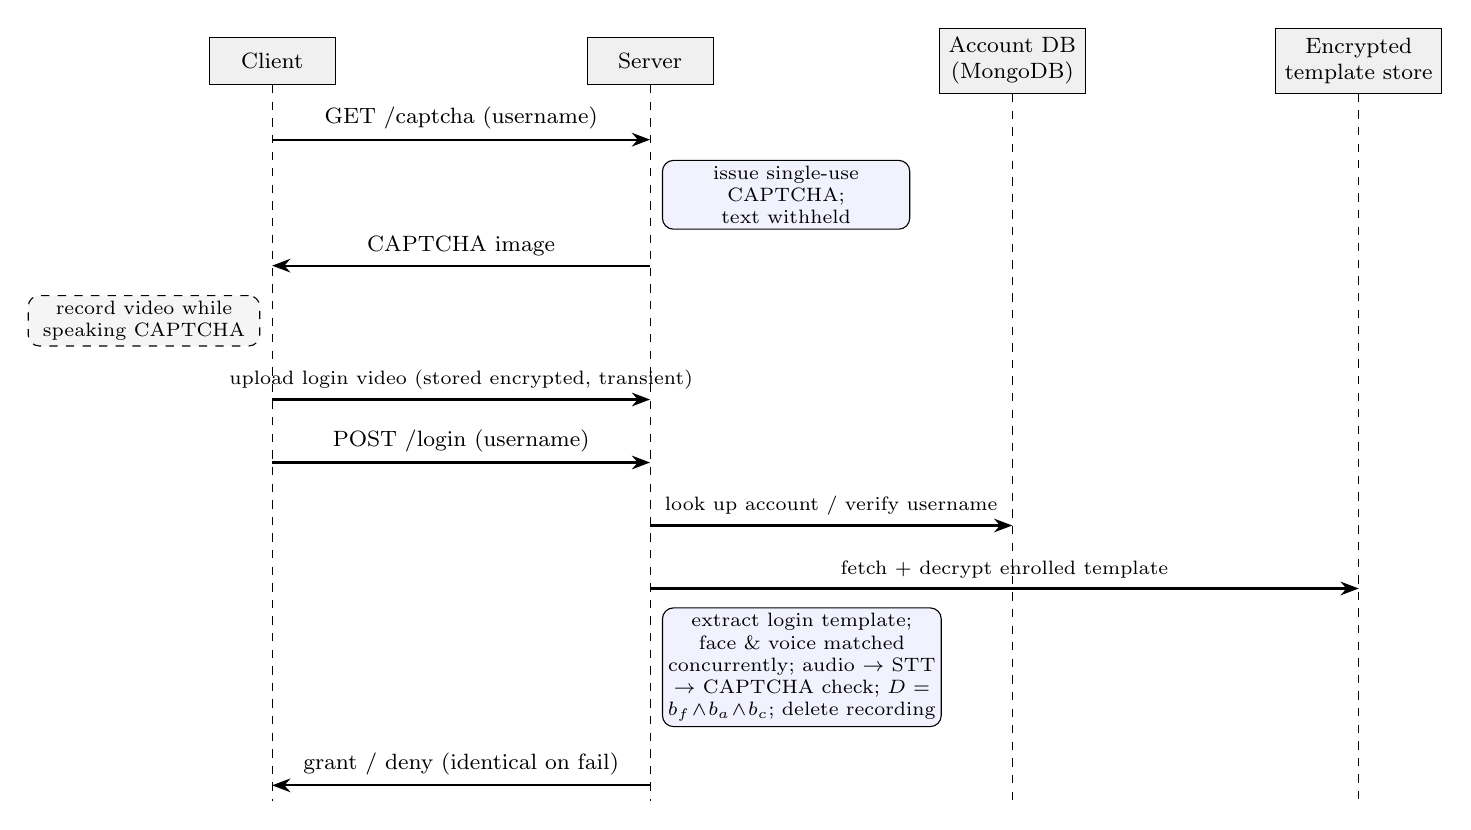
\begin{tikzpicture}[font=\footnotesize, >={Stealth[]},
  hdr/.style={draw, fill=gray!12, minimum width=16mm, minimum height=6mm, align=center},
  msg/.style={->, thick},
  note/.style={draw, fill=blue!5, rounded corners, align=center, inner sep=2pt, font=\scriptsize},
  cnote/.style={draw, dashed, fill=gray!8, rounded corners, align=center, inner sep=2pt, font=\scriptsize}]
\node[hdr] (C) at (0,0) {Client};
\node[hdr] (S) at (4.8,0) {Server};
\node[hdr] (M) at (9.4,0) {Account DB\\(MongoDB)};
\node[hdr] (T) at (13.8,0) {Encrypted\\template store};
\draw[dashed] (C.south) -- (0,-9.4);
\draw[dashed] (S.south) -- (4.8,-9.4);
\draw[dashed] (M.south) -- (9.4,-9.4);
\draw[dashed] (T.south) -- (13.8,-9.4);
\draw[msg] (0,-1) -- node[above]{GET /captcha (username)} (4.8,-1);
\node[note, anchor=west, text width=30mm] at (4.95,-1.7) {issue single-use CAPTCHA; text withheld};
\draw[msg] (4.8,-2.6) -- node[above]{CAPTCHA image} (0,-2.6);
\node[cnote, anchor=east, text width=28mm] at (-0.15,-3.3) {record video while speaking CAPTCHA};
\draw[msg] (0,-4.3) -- node[above, font=\scriptsize]{upload login video (stored encrypted, transient)} (4.8,-4.3);
\draw[msg] (0,-5.1) -- node[above]{POST /login (username)} (4.8,-5.1);
\draw[msg] (4.8,-5.9) -- node[above, font=\scriptsize]{look up account / verify username} (9.4,-5.9);
\draw[msg] (4.8,-6.7) -- node[above, font=\scriptsize]{fetch + decrypt enrolled template} (13.8,-6.7);
\node[note, anchor=west, text width=34mm] at (4.95,-7.7) {extract login template; face \& voice matched concurrently; audio $\to$ STT $\to$ CAPTCHA check; $D=b_f\wedge b_a\wedge b_c$; delete recording};
\draw[msg] (4.8,-9.2) -- node[above]{grant / deny (identical on fail)} (0,-9.2);
\end{tikzpicture}
\caption{\textcolor{blue}{Login and authentication phase (deployed). The account is looked up in MongoDB by username, while the enrolled reference is a decrypted template fetched from the \emph{separate} encrypted template store---never a stored recording. CAPTCHA issuance and video upload are distinct requests preceding the login request; the CAPTCHA text is issued server-side and withheld from the client. The three factors are evaluated concurrently and combined by the conjunctive rule of equation~(\ref{eq:fusion}); the response is identical whichever factor fails, and the login recording is deleted once the attempt resolves.}}
\label{fig:5}
\end{figure*}
\textcolor{blue}{\emph{The login-page screenshot previously shown here has been withdrawn. It displayed a four-character alphanumeric challenge, which contradicts the five-digit challenge specified in Section~\ref{sec:security}, and a \texttt{save} button absent from the current client; it also showed an identifiable participant. The login workflow is specified in the enumerated steps above and in Fig.~\ref{fig:5}.}}
\textcolor{red}{\sout{Figure: Login Steps.}}
\subsection{Authentication Phase}
The following steps are involved in the authentication phase:
{\color{blue}
\noindent The steps below supersede an earlier formulation in which each factor gated the next and the enrolled reference was read from a stored recording. Neither is the case: the enrolled reference is a template, no recording of any user exists on the server to be read, and the three factors are evaluated concurrently.
\begin{enumerate}
\item The submitted identifier is checked against the enrolled accounts.
\item The challenge issued to this identifier is retrieved and consumed, so that it cannot be reused by a subsequent attempt regardless of the outcome of this one.
\item The enrolled template and the freshly uploaded login recording are decrypted into a private working directory. Failure to decrypt or authenticate either artefact rejects the attempt immediately.
\item The login recording is reduced once to a login template, yielding its per-frame face embeddings and its speaker embedding.
\item The face and voice factors are scored against the enrolled template concurrently, by equations~(\ref{eq:face}) and~(\ref{eq:voice}).
\item Concurrently with the above, the challenge branch demultiplexes the login audio, transcribes it, and evaluates equation~(\ref{eq:captcha}). This branch depends only on the login audio, so it does not wait on the face verdict.
\item The three verdicts are combined by the conjunctive rule of equation~(\ref{eq:fusion}). On success a signed session token is issued; on failure the response is identical irrespective of which factor failed.
\item The working directory and the login recording are destroyed, whatever the outcome.
\end{enumerate}
}
\renewcommand{\algorithmicrequire}{\textbf{Input:}}
\renewcommand{\algorithmicensure}{\textbf{Output:}}


\section{Implementation and Analysis}
\subsection{Experimental Setup}
\textcolor{red}{\sout{To perform authentication, a website was developed which shows the authentication steps involved for checking the real-time working of the proposed scheme.}}\textcolor{blue}{A proof-of-concept web application was implemented to validate the feasibility of the proposed scheme under real-time acquisition. The prototype follows a client--server separation of concerns: the client is responsible only for acquisition and for presenting the server-issued challenge, while enrolment references, challenge generation, feature extraction, matching and the fusion decision of equation~(\ref{eq:fusion}) are executed on the server. Keeping the decision logic server-side is a security requirement rather than an implementation detail, since a client-side decision could be bypassed by a modified client.}
\subsubsection{Hardware Requirements}\label{sec:hw}
The Laptop used for experimenting was an Intel(R) Core(TM) i5-4210U CPU @ 1.70GHz   2.40 GHz with 8.00 GB installed RAM. The system was a 64-bit operating system, x64-based processor. The system was running Windows Operating system with edition Windows 10 Education, version 22H2, and OS build 19045.2965. The website was hosted on localhost in Chrome browser Version 114.0.5735.110 (Official Build) (64-bit). \textcolor{blue}{The functional behaviour of the scheme was verified on this machine. The timing measurements reported in Section~\ref{sec:perf} were collected on a separate host---an Intel Core i9-12900 (24 threads) with 62\,GB of RAM, running the server runtime and a local database instance---because the biometric pipeline is model-load bound and timings taken on the first machine would not be representative of the deployed configuration. The two machines are therefore not interchangeable, and the latency figures should be read against the second one.}
\subsubsection{\textcolor{red}{\protect\sout{Software Requirements}} \textcolor{blue}{Prototype Architecture}}
\textcolor{red}{\sout{The experiment requires the editor Visual Studio Code  Version 1.79.0 (user setup). The front end of the proposed scheme was built in React JS, and the back end was built in Node JS. This experiment requires Node.js 16.17.1. The database used is MongoDB, and we use MongoDB Atlas. The experiment further requires some packages like FFMPEG \cite{s1}, speechRecognition \cite{s2} library, librosa \cite{s3} for audio-related tasks and svgCaptcha \cite{s4} for server-side CAPTCHA generation.}}\textcolor{blue}{The prototype is organised as a three-tier architecture. The presentation tier is a single-page browser client that performs media capture and renders the challenge; the application tier is an event-driven server that generates the per-session CAPTCHA, orchestrates the extraction and matching pipeline and evaluates the fusion rule; and the persistence tier stores the enrolment reference associated with each unique identifier. The processing pipeline itself is realised through four functional components, each of which is independent of the specific library that implements it: a demultiplexing component that separates the video and audio streams of the acquired recording \cite{s1}, a spectral analysis component that derives the audio feature representation \cite{s3}, a speech-to-text component that produces the transcript used for challenge validation \cite{s2}, and a challenge generation component that issues an unpredictable server-side CAPTCHA per session \cite{s4}. This decomposition is deliberate: because the components interact only through the representations defined in Section~III, an individual matcher can be replaced by a stronger one without altering the system model or the decision rule. The prototype was realised as a JavaScript web application with a document-oriented store, with the media processing components invoked from the application tier. \textcolor{blue}{Key material is supplied to the application tier as three independent configuration secrets, one per domain of Section~\ref{sec:security}: a token-signing secret, a biometric-template key and an account-PII key. A deployment marked as production validates all three before the service accepts any request---each must be present and at least $32$ characters, the signing secret must not be the placeholder value carried in the source for development use, and the two storage keys must differ from each other and from the signing secret---and terminates with a diagnostic naming every violated condition if any fails, so a deployment cannot silently protect its stores with a secret intended for another purpose. The same validation guards the offline maintenance tasks, so a migration cannot be run against a production store under the wrong keys. In a development checkout the secrets may be left unset, in which case the signing secret takes a placeholder value and the storage keys are derived from it, both announced at startup; this is a convenience for local work only and is precisely the configuration the production check rejects. Key \emph{rotation} is not automated in the prototype and is discussed as an operational limitation in Section~\ref{sec:limits}.} For reproducibility the concrete stack is recorded here: a React single-page client, an Express server on Node.js~22, MongoDB for account records, and Python~3.12 for the biometric pipeline, with the face and speaker models executed on CPU through ONNX Runtime and PyTorch respectively. The pinned dependency set is distributed with the implementation.}

{\color{blue}
\subsection{\textcolor{blue}{Processing and Communication Overhead}}\label{sec:perf}
A multimodal scheme is only deployable if the additional verification it performs does not dominate the interaction, so the per-stage and end-to-end costs were measured rather than estimated. Each stage was timed over $N=5$ runs of a genuine login, on the machine described in Section~\ref{sec:hw}. All five runs returned a successful authentication with all three factors positive, so the timings are for the full success path and not for an early rejection.

\begin{table}[!htbp]
\caption{\textcolor{blue}{Measured per-stage processing time (ms, $N=5$)}}
\label{tab:stages}
\centering
\begin{tabular}{|l|r|r|r|}
\hline
\textbf{Stage} & \textbf{Mean} & \textbf{Min} & \textbf{Max} \\ \hline
Login template extraction & 12424 & 11888 & 12779 \\
Face matching & 98 & 73 & 116 \\
Voice matching & 104 & 83 & 138 \\
Audio demultiplexing & 154 & 146 & 162 \\
Speech-to-text & 2367 & 2085 & 2666 \\
\hline
\end{tabular}
\end{table}

Template extraction dominates every other stage by two orders of magnitude. The reason is architectural rather than algorithmic: it is the one stage that loads both model stacks---the face embedding network and the speaker embedding network---into a freshly created interpreter and then runs both. Matching itself is negligible on both factors, because each is a single inner product between stored vectors. The speaker-embedding migration described in Section~\ref{sec:features} in fact moved cost out of the per-login matcher, reducing voice matching from 682\,ms to 104\,ms, and into the one-time extraction stage.

\begin{table}[!htbp]
\caption{\textcolor{blue}{End-to-end authentication latency (ms, $N=5$)}}
\label{tab:e2e}
\centering
\begin{tabular}{|l|r|r|r|}
\hline
\textbf{Pipeline} & \textbf{Mean} & \textbf{Min} & \textbf{Max} \\ \hline
Cascaded (original formulation) & 15320 & 14336 & 15698 \\
Concurrent (deployed) & 13293 & 12571 & 13700 \\
\hline
\end{tabular}
\end{table}

Concurrent evaluation saves approximately 2027\,ms per authentication, a speedup of 1.15$\times$. The modest ratio is itself informative: the speedup is bounded by template extraction, because the challenge branch it overlaps with (roughly 2521\,ms of demultiplexing and transcription) is far shorter than the 12424\,ms extraction it hides behind. Further latency reduction must therefore come from amortising model loading---a resident model service rather than a fresh process per authentication---and not from additional concurrency. This is a deployment change rather than an algorithmic one and was not attempted here.

On communication cost, the client uploads one recording per attempt, which is unchanged from the original design. What changed is what the server retains: a stored template of approximately 147\,KB in place of an 11.18\,MB recording, roughly a 76-fold reduction, with a fixed 34-byte overhead for the encryption envelope. Because the authenticated cipher mode used is a stream mode, ciphertext length equals plaintext length and encryption adds no further storage cost. Upload times over a range of uplink bandwidths can be derived from the recording size but were not measured over a live link, and are therefore not reported as experimental results.
}

{\color{blue}
\subsection{\textcolor{blue}{Evaluation Scope and Limitations}}\label{sec:limits}
Because the claims of this paper should be read against the evidence that supports them, the scope of the evaluation is stated explicitly.

\emph{What was measured.} Three things were measured directly. First, the processing and communication overhead of Section~\ref{sec:perf}, over repeated runs of a genuine authentication on a single machine. Second, the score behaviour of the replaced and replacement matchers on a small set of recordings, reported in Section~\ref{sec:features} as the diagnostic that motivated each replacement. Third, the functional behaviour of the complete scheme, exercised end to end through the browser client against the deployed server.

\emph{What was not measured.} No recognition-accuracy evaluation was performed. The paper reports no false acceptance rate, no false rejection rate, no equal error rate, and no receiver operating characteristic, and no claim in it should be read as resting on such a metric. The decision thresholds were fixed from observed score separations on the available recordings, which is sufficient to place an operating point but is not a calibration against a target error rate.

\emph{Why the evaluation is bounded.} The enrolment corpus is small, and it is worth being precise about how small. The stored templates correspond to three distinct human identities. This admits exactly one genuine pairing---two separate recordings of the same person---and three impostor pairings between different people. A corpus of this size cannot support an error-rate estimate with a meaningful confidence interval, and we do not offer one. Two enrolments in the corpus are also thin, yielding only two frames containing a detectable face, which is a realistic failure mode of unconstrained capture and one that a larger study should characterise rather than exclude.

\emph{A consequence of the storage design.} The scheme's template-only storage, described in Section~\ref{sec:security} as a privacy property, has a methodological cost that should be acknowledged: because enrolment recordings are destroyed by design, the measurements taken from them cannot be recomputed later from the retained data. Reproducing them requires re-collecting the recordings. A study intending to publish accuracy results should therefore retain a separately consented evaluation corpus outside the production store, rather than relying on the deployment's own enrolments.

\emph{Reproducing the missing evaluation.} The accuracy study absent from this paper is automated rather than merely deferred. The implementation ships an evaluation harness that enumerates a corpus, extracts one template per recording using the deployed extraction path, verifies that no two recordings produce an identical template, scores every genuine and impostor pair with the deployed matchers, and emits false-acceptance and false-rejection curves, an equal error rate, and detection-error-tradeoff plots. Genuine pairs are formed only between different sessions of the same participant, never a recording against itself. The harness refuses to emit metrics from a corpus that cannot support them, which is why no numbers are reported here. Running it requires participant recordings that do not presently exist: at minimum five participants, and at least two separate sessions each, so that within-person variation across sessions is represented rather than assumed. A corpus of twenty to fifty participants with two or three sessions apiece would place the resulting rates on a footing comparable with the schemes surveyed in Section~II.

\emph{Collecting the corpus without a second protocol.} The template-only storage that gives the scheme its privacy property also erases, by design, the very recordings an accuracy study needs, since each recording is reduced to a template and discarded. To avoid a separate hand-managed collection step, the implementation provides an optional, off-by-default capture mode. When it is enabled, a participant using the application in the ordinary way---registering once and then logging in---has each uploaded recording additionally retained under the naming convention the harness consumes, with the registration providing one session and each login another, so that the different-session recordings required for genuine pairs arise from normal use rather than from a staged protocol. Because retention reverses the guarantee shown to the user, the mode is gated on \emph{per-upload consent}: the capture page displays an explicit retention notice, retention is opt-in, and the server retains a recording only when consent accompanied that specific upload, so enabling the mode never silently retains anyone who declined. Retained recordings are named by the same keyed hash used for templates, so a leak of the corpus listing discloses no identifiers; the recordings themselves remain identifying by content and must be handled under the participants' consent, and the mode is never enabled in a deployment.

\emph{Key rotation is an unmet operational requirement.} The three keys of Section~\ref{sec:security} are separated by domain and are required to be supplied independently in production, but \emph{rotating} any of them is not automated and no rotation tooling is provided. The consequences differ per domain and should be planned for before deployment. Replacing $k_{\text{bio}}$ invalidates every stored template twice over: the ciphertexts no longer authenticate under the new key, and the pseudonymous names, being keyed hashes under the same key, no longer resolve. Restoring service therefore requires decrypting each template under the retiring key and re-writing it under the new one at its newly derived name---or, if the retiring key is unavailable, re-enrolling every user, since the recordings the templates came from were destroyed by design. Replacing $k_{\text{pii}}$ requires re-encrypting the stored contact fields and recomputing the email index, without which duplicate-registration checking silently stops matching existing accounts. Replacing $k_{\text{sig}}$ is the mildest case: outstanding sessions and enrolment tokens become invalid and their holders must authenticate again, but no stored data is affected. Nothing in the current implementation performs these migrations, and a deployment that changes a key without one will fail closed---rejecting logins rather than admitting them---which is the correct failure direction but is an outage. Providing an online re-keying path, ideally with a key identifier stored alongside each record so that two key generations can coexist during a migration, is left as future work.

\emph{What this means for the comparison in Table~\ref{tab:2}.} Several schemes discussed in Section~II report equal error rates on established datasets. No comparison against those figures is made or implied here, since the corresponding quantity has not been measured for this scheme. The comparison offered is the framework comparison of Table~\ref{tab:2}, which is analytic in nature, and the contribution claimed is one of architecture, storage design and security mechanism rather than one of recognition accuracy.
}

\subsection{Analysis of the proposed scheme}
We have used the Bonneau et al. framework \cite{IEEEtran64} to analyse our proposed scheme. This comparison is done to access our scheme in terms of usability, deployability and security in comparison to existing authentication schemes. 
We have included Uname-Passwd in our comparison as it is the most easy form of authentication and preferred by normal users. Hardware token based schemes like Yubikey U2F and FIDO2 are being compared because they offer more security although they have overhead of being carried everytime and costly. Xie et al.'s CamAuth, a two factor authentication scheme which prevents various attacks Like MITM and phishing attacks and considered secure web authentication scheme is also considered for comparison. \cite{IEEEtran30} is a MFA scheme included to compare our scheme's benefits against MFA schemes. Next we compare our scheme against other multimodal biometric authentication schemes like \cite{IEEEtran63}, \cite{r1}, \cite{r4} already existing in the literature. This is described in the table \ref{tab:2} given below:
\begin{sidewaystable*}[htbp]
% \centering
\renewcommand{\arraystretch}{1.25}
\begin{tabular}{|m{5em}|m{16em}|m{4em}|m{4em}|m{4em}|m{4em}|m{4em}|m{4em}|m{4em}|m{3em}|m{4em}|}
\hline
\textbf{Aspect} & \textbf{Benefits offered}& \textbf{Uname-Passwd}&\textbf{Xie et al.}&\textbf{Abdurrah-man et al.}&\textbf{Sivakumar et al.}&\textbf{Hamad et al.}&\textbf{Kim and Hong}&\textbf{Yubikey U2F}&\textbf{FIDO2}&\textbf{Proposed scheme}\\
 \hline
     \multirow{8}{8em}{Usability} & Memorywise-effortless &\xmark & \xmark&\ymark &\ymark & \checkmark &\checkmark & \xmark& \checkmark& \checkmark \\
     \cline{2-11}
     &  Scalable-for-Users & \checkmark&\xmark& \ymark &\xmark & \checkmark & \checkmark& \ymark&\checkmark &\ymark \\
          \cline{2-11}
     & Nothing-to-Carry & \checkmark&\ymark&\checkmark &\checkmark &\checkmark &\checkmark & \xmark & \xmark&\checkmark \\
          \cline{2-11}
     & Physically-Effortless & \checkmark&\xmark&\checkmark & \xmark& \xmark & \xmark&\ymark & \checkmark&\ymark\\
          \cline{2-11}
     & Easy-to-Learn &\checkmark&\ymark& \checkmark&\checkmark & \checkmark & \checkmark&\checkmark&\checkmark & \checkmark \\
          \cline{2-11}
     & Efficient-to-Use &\checkmark&\ymark&\checkmark &\ymark & \xmark & \ymark & \checkmark&\checkmark & \ymark\\
          \cline{2-11}
     & Infrequent-Errors & \checkmark&\xmark&\checkmark & \checkmark& \ymark & \checkmark &\checkmark & \checkmark&\checkmark\\
          \cline{2-11}
     & Easy-Recovery-from-Loss & \checkmark&\ymark& \checkmark&\checkmark & \xmark & \xmark &\ymark &\xmark &\checkmark \\
     \hline
     \multirow{6}{8em}{Deployability} & Accessible & \checkmark&\xmark&\checkmark & \xmark & \ymark & \ymark& \checkmark & \checkmark&\ymark \\
     \cline{2-11}
     &  Negligible-Cost-per-User &\checkmark&\ymark&\ymark & \xmark& \xmark & \checkmark&\xmark &\ymark & \checkmark \\
          \cline{2-11}
     & Server-Compatible & \checkmark&\xmark&\ymark &\checkmark & \checkmark &\checkmark& \xmark& \xmark&\checkmark \\
          \cline{2-11}
     & Browser-Compatible & \checkmark&\ymark&\checkmark &\checkmark & \checkmark & \checkmark &\ymark & \checkmark&\checkmark\\
          \cline{2-11}
     & Mature &\checkmark& \xmark&\xmark &\xmark &\ymark &\xmark&\checkmark &\checkmark &\xmark \\
          \cline{2-11}
     & Non-proprietary & \checkmark&\checkmark& \checkmark& \checkmark&\checkmark & \checkmark&\xmark & \checkmark&\checkmark\\
          \hline
    \multirow{9}{8em}{Security} & Resilient-to-Physical-Observation&\xmark &\checkmark&\checkmark  &\checkmark & \checkmark &\checkmark & \checkmark&\checkmark &\checkmark \\
     \cline{2-11}
     & Resilient-to-Targeted-Impersonation &\xmark&\checkmark&  &\checkmark &\checkmark&\ymark&\checkmark &\checkmark &\checkmark \\
          \cline{2-11}
     & Resilient-to-Throttled-Guessing &\xmark&\checkmark& \checkmark& \checkmark&\checkmark& \checkmark&\checkmark&\checkmark & \checkmark \\
          \cline{2-11}
     & Resilient-to-Unthrottled-Guessing &\xmark&\checkmark& \checkmark& \checkmark&\checkmark&\checkmark & \checkmark&\checkmark & \checkmark\\
          \cline{2-11}
     & Resilient-to-Internal-Observation &\xmark&\xmark& \checkmark&\checkmark & \checkmark &\checkmark& \ymark&\checkmark &\checkmark \\
          \cline{2-11}
     & Resilient-to-Leaks-from-Other-Verifiers & \checkmark&\checkmark& 
     \checkmark&\xmark &\checkmark& \checkmark &\ymark&\checkmark &\checkmark\\
          \cline{2-11}
     & Resilient-to-Phishing & \xmark&\xmark& \xmark&\checkmark &\ymark&\ymark &\checkmark & \checkmark&\checkmark \\
     \cline{2-11}
      & Resilient-to-Theft & \checkmark&\checkmark& \checkmark& \checkmark& \checkmark &\checkmark    &\checkmark&\xmark &\checkmark \\
     \cline{2-11}
      & No-trusted-Third-Party &\checkmark&\checkmark&\checkmark & \checkmark& \checkmark& \checkmark&\xmark&\checkmark & \textcolor{red}{\sout{\checkmark}}\textcolor{blue}{\xmark} \\
     \cline{2-11}
      & Require-Explicit-Consent &\checkmark&\checkmark& \checkmark& \checkmark& \checkmark& \checkmark&\checkmark&\checkmark &\checkmark \\
     \cline{2-11}
      & Unlinkable & \checkmark&\checkmark &\checkmark &\checkmark & \checkmark&\checkmark &\checkmark& \checkmark&\checkmark \\
     \hline
     & \textit{Benefit offered count} &\textbf{\textit{18}} &\textbf{\textit{10}}&\textbf{\textit{18}}&\textbf{\textit{17}}&\textbf{\textit{17}}&\textbf{\textit{18}}&\textbf{\textit{13}}&\textbf{\textit{20}}&\textbf{\textit{\textcolor{red}{\sout{20}}\textcolor{blue}{19}}}\\
     \hline
     
\end{tabular}
    \caption{Analysis of the Proposed Scheme where
    \checkmark : Benefit offered by the scheme,
    \ymark: Partial benefit offered by the scheme
    \xmark: Benefit not offered by the scheme.
    \textcolor{blue}{The ratings in this table are analytic, following the framework's own methodology; they are reasoned from each scheme's design and are not empirical measurements. In particular the security ratings for the proposed scheme are not backed by a recognition-accuracy study, and the entries that would depend on one are argued from the conjunctive decision rule rather than from measured error rates. The \emph{No-trusted-Third-Party} rating for the proposed scheme is revised downward: the challenge factor transcribes the spoken utterance through an external speech-to-text service, so the login audio leaves the verifier's trust boundary and a third party is relied upon for the availability and correctness of that factor. Replacing it with an on-premises recogniser would restore the benefit and is identified as future work. A registration acknowledgement email is additionally dispatched through a hosted SMTP provider; it is an auxiliary notification sent on a best-effort basis after an account is created and is not part of the authentication workflow, so it does not bear on this rating, though a self-hosted mail relay would remove even that auxiliary dependency. The \emph{Unlinkable} rating refers to the biometric template store, whose file names are keyed hashes; it does not assert unlinkability of the separate account database, which is discussed in Section~\ref{sec:security}.}}
    \label{tab:2}
\end{sidewaystable*}
\section{Conclusions}
This paper proposes a multimodal biometric-based authentication system that enhances usability by allowing parallel acquisition of biometric samples. This scheme relates to a user authentication system based on a dynamic CAPTCHA and a real-time single Video input to develop a multimodal biometric authentication system. Through our research, we have achieved the following key findings:
\begin{enumerate}
    \item \textcolor{red}{\sout{We have found that no proposed scheme involves the parallel acquisition of biometric samples and checking liveliness. We have designed a scheme which provides the same.}}\textcolor{blue}{Prior multimodal schemes generally acquire each trait through a dedicated sensor and seldom bind acquisition to a per-session challenge; the proposed scheme instead couples parallel acquisition of multiple biometric samples from a single sensor with a challenge-bound liveness cue, and we have designed and implemented a scheme which provides both.}
    \item The schemes already present in the literature in the field of multimodal biometrics are costly due to the use of expensive devices, which hinders their applicability by users. Our scheme is cost-effective.
\end{enumerate}
\textcolor{red}{\sout{These findings provide valuable insights into multimodal biometric authentication schemes and contribute to the existing body of knowledge in several ways. They offer a deeper understanding of the problem and lay the foundation for further advancements and improvements in the future.}}\textcolor{blue}{The scheme was assessed along two axes: qualitatively against the Bonneau et al. framework, which situates it with respect to existing usability, deployability and security benefits, and quantitatively through the processing-delay measurements of Section~\ref{sec:perf}. Neither axis characterises recognition accuracy, which is treated as a limitation below.}\\
\textcolor{red}{\sout{Moreover, our research has highlighted the significance of multimodal biometrics and its impact on authentication. By addressing and investigating this aspect, we have made significant progress towards advancing the field and filling the existing research gaps.}}\textcolor{blue}{The limitations of this work are set out in full in Section~\ref{sec:limits} and are summarised here. Recognition accuracy is not characterised: no false acceptance, false rejection or equal error rate is reported, and the thresholds in use fix an operating point on a small corpus rather than calibrating against a target error rate. The timing results come from repeated runs of one account on a single machine, and their dominant stage is a model-loading cost that a resident model service would largely remove. The liveness argument rests on the unpredictability of the challenge rather than on an explicit presentation-attack detector. The challenge factor depends on an external speech-to-text service, which places the login audio outside the verifier's trust boundary. Reporting error rates over a multi-subject corpus, adding a presentation-attack detection stage, and substituting an on-premises recogniser are the natural directions for future work.}
\textcolor{blue}{The frame- and audio-extraction stages and the speech-to-text stage, previously shown as implementation screenshots, are described in the text of this section and in Algorithm~\ref{alg:extract}: frames are sampled uniformly across the recording, the audio track is demultiplexed from the same recording, and the login audio is transcribed for challenge validation. The matcher outputs, previously shown as terminal listings, are consolidated in Table~\ref{tab:scores}.}

\begin{table}[!htbp]
\caption{\textcolor{blue}{Deployed matcher scores on the available recordings (cosine similarity; a factor is accepted when its score reaches the threshold). A genuine pair is two separate recordings of one subject; an impostor pair is two different subjects. These are the diagnostics of Section~\ref{sec:features} that motivated each matcher replacement, not an accuracy evaluation; no error rate is claimed from them. They replace the superseded perceptual-hash and MFCC/Euclidean matchers.}}
\label{tab:scores}
\centering
{\small
\begin{tabular}{|p{3.05cm}|c|c|c|}
\hline
\textbf{Factor (deployed matcher)} & \textbf{Genuine} & \textbf{Impostor} & \textbf{Thresh.} \\ \hline
Face: median per-frame cosine (Alg.~\ref{alg:face-new}) & 0.8385 & 0.0928 & $\tau_f{=}0.35$ \\ \hline
Voice: ECAPA-TDNN speaker cosine (Alg.~\ref{alg:voice-new}) & 0.455 & 0.090 & $\tau_a{=}0.30$ \\ \hline
\end{tabular}}
\end{table}
\begin{table}
\caption{NOTATIONS AND ABBREVIATIONS}
\label{tab:notations}
\begin{tabular}{|c|l|}
\hline
\textbf{Notation} & \textbf{Description} \\ \hline
$Uname$ & Username \\
$V_r$ & \textcolor{blue}{Transient} video captured during registration \textcolor{blue}{(destroyed after extraction)} \\
$V_l$ & Video captured during login phase \\
$F_l$ & Frames extracted from login video  \\
\textcolor{blue}{$A_l$} & \textcolor{blue}{Audio demultiplexed from the login recording}\\
$P_1,P_2$ & Perceptual Hash value \textcolor{blue}{(original design)}\\
$MFCC$ &  Mel-frequency Cepstral Coefficients \textcolor{blue}{(original design)} \\
$pHash$ & Perceptual Hashing Algorithm for images \textcolor{blue}{(original design)}\\
\textcolor{blue}{$e^{f}_r$, $e^{f}_{l,i}$} & \textcolor{blue}{Enrolled face embedding; $i$-th login frame embedding}\\
\textcolor{blue}{$e^{a}_r$, $e^{a}_l$} & \textcolor{blue}{Enrolled and login speaker embeddings}\\
\textcolor{blue}{$\tau_f$, $\tau_a$} & \textcolor{blue}{Face and voice acceptance thresholds}\\
\textcolor{blue}{$b_f,b_a,b_c$} & \textcolor{blue}{Face, voice and challenge factor decisions}\\
\textcolor{blue}{$D$} & \textcolor{blue}{Fused authentication decision}\\
\textcolor{blue}{$C$, $\mathcal{N}(\cdot)$} & \textcolor{blue}{Issued CAPTCHA; normalization map}\\
\textcolor{blue}{$T(A_l)$} & \textcolor{blue}{Ranked transcription hypotheses for $A_l$}\\
\textcolor{blue}{$T_r$, $T_l$} & \textcolor{blue}{Enrolled template; login template}\\
\textcolor{blue}{$E$, $\sigma$} & \textcolor{blue}{Enrolment token; session token}\\
\textcolor{blue}{$k_{\text{sig}}$} & \textcolor{blue}{Token-signing key (sessions, enrolment)}\\
\textcolor{blue}{$k_{\text{bio}}$} & \textcolor{blue}{Biometric template key (AES-256-GCM, HMAC names)}\\
\textcolor{blue}{$k_{\text{pii}}$} & \textcolor{blue}{Account-PII key (AES-256-GCM, email index)}\\
\textcolor{blue}{$\mathcal{H}_{k}(\cdot)$} & \textcolor{blue}{Keyed hash (HMAC) under key $k$}\\
\textcolor{blue}{$\mathcal{N}_e(\cdot)$} & \textcolor{blue}{Email normalization (trim, lowercase)}\\
\hline
\end{tabular}
\end{table}

\textcolor{blue}{\emph{The three algorithms previously given here---a login-and-authentication procedure that cascaded the factors and read the enrolled recording from disk, a frame matcher based on perceptual hashing and Hamming distance, and an audio matcher based on mean pairwise Euclidean distance between MFCC matrices---have been withdrawn. They describe an architecture that is no longer the one implemented: the enrolled reference is a template rather than a recording, the two matchers were replaced for the reasons measured in Section~\ref{sec:features}, and the factors are evaluated concurrently rather than in a cascade. The pseudocode below specifies the deployed system end to end, in the order in which the phases occur. Algorithms~\ref{alg:register}--\ref{alg:auth} give the three phases of Section~\ref{sec:model}; Algorithms~\ref{alg:face-new}--\ref{alg:fusion} give the per-factor decisions and the fusion rule invoked by Algorithm~\ref{alg:auth}; Algorithm~\ref{alg:extract} is the extraction procedure shared by enrolment and login.}}

{\color{blue}
\begin{algorithm*}[!tbp]
\caption{\textcolor{blue}{User Registration / Enrolment}}\label{alg:register}
\begin{algorithmic}[1]
\Require identifier $u$; email address $m$; optional avatar; live recording capability at the client
\Ensure an encrypted template stored under $\mathcal{H}_{k_{\text{bio}}}(u)$, or a rejection
\Statex \emph{Phase 1 --- account creation (first request)}
\State client submits $(u, m, \text{avatar})$ to the server
\State \textbf{if} $u$ does not match the permitted identifier character class \textbf{then reject}
\State \textbf{if} $m$ is empty \textbf{then reject}; $\quad \texttt{idx} \gets \mathcal{H}_{k_{\text{pii}}}\big(\mathcal{N}_e(m)\big)$ \Comment{non-emptiness is the only check on the address; it is matched through its index, never by comparing stored addresses}
\State $a_u \gets$ account holding $u$; $\quad a_m \gets$ account holding $\texttt{idx}$
\State \textbf{if} $a_u$ or $a_m$ holds a stored template \textbf{then reject} \Comment{an enrolment is never displaced}
\State delete $a_u$ and $a_m$ if present \Comment{both conflicts are resolved before either deletion, so a request that will be rejected destroys nothing; an account with no template was never bound to any biometrics, so its identifier is released}
\State create the account record for $(u, \texttt{idx}, m, \text{avatar})$ by \textsc{SealAccount} \Comment{Algorithm~\ref{alg:pii}: identifier readable, contact fields under $k_{\text{pii}}$}
\State $E \gets \mathrm{Sign}_{k_{\text{sig}}}\big(\{\texttt{username}{=}u,\ \texttt{purpose}{=}\text{enrol}\},\ \texttt{ttl}{=}10\ \text{min}\big)$
\Statex \Comment{the token carries the identifier and the purpose and nothing else---no account identifier, no nonce, and no server-side record of issuance---so it is a bearer credential that any holder may present until it expires}
\State return $E$ to the client
\Statex \emph{Phase 2 --- enrolment (second request)}
\State the client renders a challenge locally; the user records $V_r$ while speaking it
\Statex \Comment{this registration challenge is generated at the client and is never verified: it elicits natural speech for the voice template and is not an authentication factor}
\State client uploads $V_r$, presenting $E$ as a bearer token
\State \textbf{if} $E$ fails to verify under $k_{\text{sig}}$, or its purpose is not enrolment, or it has expired, or its identifier claim is malformed \textbf{then reject}; \textbf{otherwise} $u' \gets$ the identifier claim of $E$
\Statex \Comment{a session token is refused here because its purpose claim differs, so a stolen session cannot re-key an account}
\State \textbf{if} the uploaded filename does not match the expected pattern \textbf{then reject} \Comment{the filename is shape-checked only; the enrolled identity is $u'$, taken from the verified token and never from the filename}
\State $a \gets$ the account whose identifier is $u'$
\Statex \Comment{the lookup is by identifier alone, because $E$ names no account instance: an account created after $E$ was issued, but holding the same identifier, satisfies it}
\State \textbf{if} $a$ does not exist \textbf{then reject} \Comment{$E$ outlives an account that was rolled back; no template is stored for an identifier that no account holds}
\State \textbf{if} a template is already stored under $\mathcal{H}_{k_{\text{bio}}}(u')$ \textbf{then reject}
\Statex \Comment{an enrolment is final. $E$ is \emph{not} consumed by use and stays valid for the remainder of its ten minutes, so it is this check, rather than single-use semantics, that prevents a valid token from replacing a stored template}
\State \textbf{if} evaluation capture is enabled \emph{and} this upload carried consent \textbf{then} retain a copy of $V_r$ \Comment{off by default; when active it suspends the storage property asserted below, and is used only for consented corpus collection (Section~\ref{sec:limits})}
\State write $V_r$ into a private working directory $W$
\State $T_r \gets \textsc{ExtractTemplate}(V_r)$ \Comment{Algorithm~\ref{alg:extract}, run as a subprocess under a timeout; a timeout counts as failure}
\If{$T_r = \textbf{failure}$} \Comment{no usable face, unreadable recording, or no usable audio}
    \State destroy $W$; delete the account $a$ \Comment{the rollback is itself conditioned on no template being present, and a failure to delete is logged while the rejection is still returned}
    \State \Return rejection \Comment{fail closed: no template is stored, so no account holds an unusable reference}
\EndIf
\State attempt $c \gets \mathrm{Enc}^{\text{AES-256-GCM}}_{k_{\text{bio}}}(T_r)$ and write $c$ under the pseudonymous name $\mathcal{H}_{k_{\text{bio}}}(u')$
\Statex \Comment{the biometric key, never the token-signing key; the keyed name keeps every plaintext identifier out of the template store}
\State destroy $W$, and with it $V_r$ and every plaintext copy of $T_r$ \Comment{performed whatever the outcome of the previous step: template-only storage, the recording is never persisted}
\If{the storage attempt failed}
    \State \Return failure, leaving $a$ in place \Comment{this path performs no rollback, unlike an extraction failure: the account remains with no template and is released by step~6 of a later registration}
\EndIf
\State \Return registration successful
\Statex \Comment{$E$ is not invalidated here and remains valid until it expires; a further registration for $u'$ is now refused at step~5, because the account holds a stored template}
\end{algorithmic}
\end{algorithm*}

\begin{algorithm}[!tbp]
\caption{\textcolor{blue}{Login and Challenge Issuance}}\label{alg:challenge}
\begin{algorithmic}[1]
\Require identifier $u$ submitted at the client
\Ensure a fresh single-use challenge bound to $u$, and an uploaded login recording $V_l$
\State \textbf{if} $u$ does not match the permitted identifier character class \textbf{then reject}
\State $C \gets$ five symbols drawn uniformly at random from the challenge alphabet $\Sigma$ \Comment{$\Sigma$ is the five-digit decimal alphabet of Section~\ref{sec:security}}
\State bind and store $(u, C, \texttt{expiry} = \text{now} + 5\ \text{minutes})$ in the server-side challenge store
\State render $C$ as an image and transmit \emph{only} the rendered image to the client
\Statex \Comment{the expected string never leaves the server; a client that knew it could satisfy the factor without a live utterance}
\State the user records $V_l$ while speaking the displayed challenge
\State client uploads $V_l$ under a filename that carries the identifier
\State \textbf{if} the uploaded filename does not match the expected pattern \textbf{then reject}; \textbf{otherwise} $u' \gets$ the identifier embedded in that filename
\Statex \Comment{this endpoint, unlike enrolment (Algorithm~\ref{alg:register}), has no token with which to bind the upload: the caller has not authenticated and is precisely in the act of attempting to, so the account whose recording slot is written is named by the client-supplied filename. Binding to a live attempt is supplied by the challenge test below rather than by a credential}
\State \textbf{if} no issued, unexpired challenge exists for $u'$ \textbf{then} reject the upload \Comment{a recording cannot be submitted outside a live login attempt; the challenge is checked here but not yet consumed}
\State \textbf{if} evaluation capture is enabled \emph{and} this upload carried consent \textbf{then} retain a copy of $V_l$ \Comment{off by default; when active it suspends the transience asserted below, and is used only for consented corpus collection (Section~\ref{sec:limits})}
\State store $V_l$ encrypted under $k_{\text{bio}}$ in a transient location \Comment{two independent branches of Algorithm~\ref{alg:auth} consume it; it belongs to the biometric domain and is deleted once the attempt resolves}
\State the client requests authentication for $u$ \Comment{continues at Algorithm~\ref{alg:auth}}
\end{algorithmic}
\end{algorithm}

\begin{algorithm}[!tbp]
\caption{\textcolor{blue}{Concurrent Authentication (deployed)}}\label{alg:auth}
\begin{algorithmic}[1]
\Require identifier $u$; uploaded login recording $V_l$
\Ensure session token on success, or a rejection that is identical across the three factors
\State \textbf{if} no account exists for $u$, or $u$ fails identifier validation, \textbf{then reject}
\State $C \gets \textsc{TakeChallenge}(u)$ \Comment{retrieves \emph{and} consumes: single-use, whether or not this attempt succeeds; $C = \bot$ if none was issued or it expired}
\State create a private working area $W$
\State $T_r \gets \mathrm{Dec}_{k_{\text{bio}}}\big(\text{store}[\mathcal{H}_{k_{\text{bio}}}(u)]\big)$ into $W$; $\quad V_l \gets \mathrm{Dec}_{k_{\text{bio}}}(\text{transient upload})$ into $W$ \Comment{both artefacts belong to the biometric domain and use its key alone}
\State \textbf{if} either decryption or its authentication tag fails \textbf{then} destroy $W$ and \textbf{reject} \Comment{fail closed on a missing or tampered artefact}
\Parallel
\Branch{$\mathcal{B}_{\text{bio}}$}
    \State $T_l \gets \textsc{ExtractTemplate}(V_l)$ \Comment{Algorithm~\ref{alg:extract}; yields $\{e^{f}_{l,i}\}$ and $e^{a}_{l}$}
    \State \textbf{if} $T_l = \textbf{failure}$ \textbf{then} $b_f \gets 0$; $b_a \gets 0$
    \State \textbf{else} evaluate concurrently:
    \Statex \quad\quad $b_f \gets \textsc{VerifyFace}(T_r, T_l)$ \Comment{Algorithm~\ref{alg:face-new}}
    \Statex \quad\quad $b_a \gets \textsc{VerifySpeaker}(T_r, T_l)$ \Comment{Algorithm~\ref{alg:voice-new}}
\EndBranch
\Branch{$\mathcal{B}_{\text{chal}}$}
    \State $T(A_l) \gets$ the transcription stage of \textsc{VerifyChallenge}$(V_l)$ \Comment{Algorithm~\ref{alg:captcha}, steps 1--3; depends only on the login audio, so it does not wait on the face or speaker verdict}
\EndBranch
\EndParallel
\State wait until $b_f$, $b_a$ and $T(A_l)$ are all available \Comment{the conjunction is \emph{not} evaluated lazily: no factor gates another}
\State $b_c \gets$ the comparison stage of \textsc{VerifyChallenge}$(T(A_l), C)$ \Comment{Algorithm~\ref{alg:captcha}, steps 4--6: the branch produces the hypotheses concurrently, and the verdict against $C$ is formed once the branches have joined}
\State $D \gets \textsc{Fuse}(b_f, b_a, b_c)$ \Comment{Algorithm~\ref{alg:fusion}}
\State record $(b_f, b_a, b_c)$ in the server log only
\If{$D = 1$}
    \State $\sigma \gets \mathrm{Sign}_{k_{\text{sig}}}\big(\{\texttt{account},\ \texttt{username}{=}u\},\ \texttt{ttl}{=}24\ \text{h}\big)$ \Comment{session token, signed under the token key and carrying the account reference and identifier; the storage keys play no part here}
    \State $r \gets (\textsc{granted}, \sigma)$
\Else
    \State $r \gets \textsc{denied}$ \Comment{a single response, identical whichever factor failed and identical to the response given when decryption failed at step~5; the per-factor outcome is never disclosed. The rejections at step~1, which precede any factor evaluation, are distinguishable from it}
\EndIf
\State destroy $W$ and delete the transient login recording, whatever the outcome
\State \Return $r$
\end{algorithmic}
\end{algorithm}

\begin{algorithm}[!tbp]
\caption{\textcolor{blue}{\textsc{VerifyFace}: face verification}}\label{alg:face-new}
\begin{algorithmic}[1]
\Require enrolled face reference $e^{f}_r$ from $T_r$; login frame embeddings $\{e^{f}_{l,i}\}_{i=1}^{n}$ from $T_l$
\Ensure face verdict $b_f$
\State \textbf{if} $e^{f}_r$ is absent or $n = 0$ \textbf{then return} error \Comment{fail closed}
\For{$i = 1$ to $n$} \Comment{$n \leq 12$: twelve frames are sampled uniformly across the recording}
    \State $s_i \gets \big\langle e^{f}_{r},\, e^{f}_{l,i} \big\rangle$ \Comment{both vectors are L2-normalized 512-d deep embeddings, so $s_i$ is a cosine similarity}
\EndFor
\State $s \gets \operatorname{median}(s_1,\dots,s_n)$
\Statex \Comment{the median, not the mean: a minority of degraded frames (motion blur, partial pose, transient occlusion) cannot move the verdict}
\If{$s \geq \tau_f$} \Comment{deployed threshold $\tau_f = 0.35$}
    \State $b_f \gets 1$
\Else
    \State $b_f \gets 0$
\EndIf
\State \Return $b_f$
\end{algorithmic}
\end{algorithm}

\begin{algorithm}[!tbp]
\caption{\textcolor{blue}{\textsc{VerifySpeaker}: voice verification}}\label{alg:voice-new}
\begin{algorithmic}[1]
\Require enrolled speaker embedding $e^{a}_r$ from $T_r$; login speaker embedding $e^{a}_l$ from $T_l$
\Ensure speaker verdict $b_a$
\Statex \Comment{both embeddings are stored quantities: the enrolled one was computed once at registration, the login one by Algorithm~\ref{alg:extract}. No registration audio exists on the server to be re-extracted.}
\State \textbf{if} either template carries no speaker embedding \textbf{then return} error \Comment{a legacy template cannot be scored; re-enrolment is required}
\State $e^{a}_r \gets e^{a}_r / \lVert e^{a}_r \rVert$; \quad $e^{a}_l \gets e^{a}_l / \lVert e^{a}_l \rVert$
\State $s \gets \big\langle e^{a}_{r},\, e^{a}_{l} \big\rangle$ \Comment{cosine similarity of two 192-d speaker embeddings}
\If{$s \geq \tau_a$} \Comment{deployed threshold $\tau_a = 0.30$}
    \State $b_a \gets 1$
\Else
    \State $b_a \gets 0$
\EndIf
\State \Return $b_a$
\end{algorithmic}
\end{algorithm}

\begin{algorithm}[!tbp]
\caption{\textcolor{blue}{\textsc{VerifyChallenge}: spoken-challenge verification}}\label{alg:captcha}
\begin{algorithmic}[1]
\Require login recording $V_l$; challenge $C$ retrieved and consumed by Algorithm~\ref{alg:auth}
\Ensure challenge verdict $b_c$
\State $A_l \gets$ audio track demultiplexed from $V_l$
\State $T(A_l) \gets$ ranked transcription hypotheses returned by the speech-to-text stage
\State \textbf{if} demultiplexing or transcription failed \textbf{then} $T(A_l) \gets \emptyset$
\State \textbf{if} $C = \bot$ or $T(A_l) = \emptyset$ \textbf{then return} $b_c \gets 0$
\Statex \Comment{fail closed when no challenge was issued for this identifier or it expired. The test is applied here rather than before step~1: the transcription stage runs on the login audio regardless, so an attempt carrying no live challenge performs the same work as one that does and is rejected on the same verdict}
\State $b_c \gets \mathbb{I}\big[\exists\, t \in T(A_l): \mathcal{N}(t) = \mathcal{N}(C)\big]$ \Comment{equation~(\ref{eq:captcha})}
\Statex \Comment{\emph{any} hypothesis may carry the correct reading: the top-ranked alternative for a spoken digit string is frequently a sound-alike word. $\mathcal{N}(\cdot)$ normalizes case and separators and maps spelled-out number words to numerals, so a correct utterance is not rejected for orthographic reasons.}
\State \Return $b_c$
\end{algorithmic}
\end{algorithm}

\begin{algorithm}[!tbp]
\caption{\textcolor{blue}{\textsc{Fuse}: decision-level AND fusion}}\label{alg:fusion}
\begin{algorithmic}[1]
\Require face verdict $b_f$, speaker verdict $b_a$, challenge verdict $b_c$, each in $\{0,1\}$
\Ensure fused decision $D$
\State $D \gets b_f \wedge b_a \wedge b_c$ \Comment{equation~(\ref{eq:fusion})}
\State \Return $D$
\Statex \Comment{$D = 1$, and access is granted, only when $b_f = b_a = b_c = 1$; $D = 0$ otherwise. The rule is conjunctive by design: the compromise or failure of any single factor is sufficient to deny authentication, so no one modality can produce a positive decision on its own. The caller returns one rejection response for every $D = 0$ case, so which factor was zero is never disclosed to the client.}
\end{algorithmic}
\end{algorithm}

\begin{algorithm}[!tbp]
\caption{\textcolor{blue}{\textsc{ExtractTemplate}: shared extraction procedure}}\label{alg:extract}
\begin{algorithmic}[1]
\Require recording $V$
\Ensure template $T = \{e^{f}, \{e^{f}_{i}\}, e^{a}\}$, or \textbf{failure}
\If{the container reports a frame count}
    \State sample $m = 12$ frames uniformly across $V$
\Else
    \State read $V$ sequentially, retaining every fifth frame, until $12$ embeddings have been obtained
    \Statex \quad \Comment{browser-produced containers frequently report no frame count, so uniform sampling has no index range to span; the stride keeps the retained frames from being one contiguous burst}
\EndIf
\For{each retained frame}
    \State detect faces; if several are present, retain the largest
    \State $e^{f}_{i} \gets$ L2-normalized 512-d deep face embedding of the retained face
\EndFor
\If{no frame yielded a face}
    \State \Return \textbf{failure} \Comment{fail closed: at enrolment no template is stored, at login the biometric verdicts are $0$}
\EndIf
\State $e^{f} \gets \mathrm{normalize}\big(\mathrm{mean}_i\, e^{f}_{i}\big)$ \Comment{used as the enrolled face reference; at login the per-frame set $\{e^{f}_{i}\}$ is what Algorithm~\ref{alg:face-new} scores}
\State demultiplex the audio track of $V$ and resample to 16\,kHz mono
\If{audio shorter than one second}
    \State \Return \textbf{failure}
\EndIf
\State $e^{a} \gets \mathrm{normalize}\big(\text{speaker-embedding network}(\text{audio})\big)$ \Comment{192-d ECAPA-TDNN embedding}
\State \Return $T$
\end{algorithmic}
\end{algorithm}

\begin{algorithm}[!tbp]
\caption{\textcolor{blue}{\textsc{SealAccount}: account-record storage}}\label{alg:pii}
\begin{algorithmic}[1]
\Require identifier $u$; email address $m$; optional profile fields $p = (\text{first},\text{last},\text{mobile},\text{address},\text{avatar})$
\Ensure an account record in which only $u$ is readable
\State store $u$ in plaintext \Comment{the login lookup key; the client submits it on every request, so sealing it would conceal nothing and would put a blind index on the authentication path}
\State $\texttt{idx} \gets \mathcal{H}_{k_{\text{pii}}}\big(\mathcal{N}_e(m)\big)$ \Comment{keyed index over the normalized address: deterministic, so duplicate registration is still detected; not invertible, so no stored address is read to detect it}
\State store $\texttt{idx}$, and enforce uniqueness on it rather than on the address \Comment{ciphertext cannot carry uniqueness: a random IV makes two equal addresses differ byte for byte}
\State store $\mathrm{Enc}^{\text{AES-256-GCM}}_{k_{\text{pii}}}(m)$
\For{each supplied field $f \in p$}
    \State store $\mathrm{Enc}^{\text{AES-256-GCM}}_{k_{\text{pii}}}(f)$ \Comment{account domain key throughout; $k_{\text{bio}}$ and $k_{\text{sig}}$ are never used here}
\EndFor
\Statex \Comment{this record is held in the account database, which contains no template and no template name; the template store (Algorithm~\ref{alg:register}) correspondingly contains no plaintext identifier}
\Statex \Comment{on read, the sealed fields are opened and returned, $\texttt{idx}$ is withheld from the client, and a field failing its authentication tag rejects the read rather than returning a partial record. The profile endpoint of the prototype is not access-controlled: it opens the record for any caller naming the identifier, so the protection this procedure provides is confidentiality against a compromise of the database itself, not an access-control property of the running service}
\end{algorithmic}
\end{algorithm}
}
\subsection{Frame Extraction and Frame Matching}
\textcolor{blue}{\emph{The remainder of this subsection describes the perceptual-hash matcher as originally specified. It is retained for reference and comparison; the deployed face factor is the embedding matcher of Section~\ref{sec:features} and Algorithm~\ref{alg:face-new}, which replaced it because the measurements reported there showed the perceptual hash false-rejecting a genuine user.}}
\textcolor{red}{\sout{OpenCV, short for Open Source Computer Vision Library, is a powerful and widely used library for real-time computer vision applications. We are using OpenCV's cv2.VideoCapture class available in python to extract frames from videos.}}\textcolor{blue}{Frames are obtained by uniform temporal sampling of the recording, so that the sampled set spans the whole clip rather than a single burst.}
\par { We are calculating $pHash$ of each frame captured from video during frame extraction step. A perceptual hash is a compact digital fingerprint derived from a multimedia file (image, audio, video). Unlike cryptographic hashes (like MD5 or SHA256), it focuses on capturing the perceptual similarity of the content, not the exact data. This means that even if an image is slightly modified (e.g., resized, compressed, brightness adjusted), the perceptual hash remains similar, as long as the overall visual content is preserved. Perceptual hashing algorithms typically involve these steps:
\begin{itemize}
    \item Preprocessing:The multimedia file might undergo basic transformations (e.g., resizing, color space conversion) to ensure consistency.
    \item Feature Extraction: The algorithm extracts features that capture the essence of the content. For images, these features include Edges, colors, spatial patterns, textures.
    \item Hashing Function: The extracted features are fed into a hashing function that generates a compact digest (the perceptual hash). This function is designed to produce similar hashes for perceptually similar content. 
\end{itemize}
$pHash$ is the perceptual hashing algorithm popularly used for images.
We calculate hamming distance between the phash calculated by first converting these phashes to binary strings to decide the frame matching result. Hamming Distance compares two binary strings of equal length (like phash outputs).
It calculates the number of positions where the corresponding bits differ (mismatches). Lower Hamming distance indicates higher similarity between the phashes. 
}
\subsection{Audio Extraction and Audio Matching}
We are using \textcolor{red}{\sout{FFMPEG frame work to extract frames from}}\textcolor{blue}{stream demultiplexing to extract the audio track from the}  video captured during registration and login phase. \textcolor{blue}{The audio track is demultiplexed without re-encoding where possible. Two points differ from the original description. First, no registration audio is demultiplexed at login: the enrolled voice reference is the speaker embedding computed once at enrolment, so only the login recording is processed. Second, the demultiplexed audio is written to a private temporary location that is destroyed when the attempt resolves, rather than to a persistent per-user file.}
\par \textcolor{blue}{\emph{The remainder of this subsection describes the MFCC matcher as originally specified. It is retained for reference and comparison; the deployed voice factor is the speaker-embedding matcher of Section~\ref{sec:features} and Algorithm~\ref{alg:voice-new}, which replaced it because the measurements reported there showed the MFCC statistic failing to separate speakers at any threshold.}}
\par {For audio matching, we are using Librosa library available in python. It is a versatile tool for working with audio data in various analysis and processing tasks. We use $librosa.load$ to load audio files. It Loads an audio file from disk (specified audio path) into a NumPy array representing the audio waveform. We then compute Mel-frequency cepstral coefficients (MFCCs) from an audio signal. MFCCs are a popular feature representation in audio analysis, capturing the spectral envelope of the sound. One of the parameters in MFCC calculation is n\_mfcc  which represents the number of MFCC coefficients to compute. We have set this parameter value to 13. This determines the dimensionality of the output feature vector.MFCCs are widely used in various audio processing tasks, including - Speech recognition, Speaker identification. We compute the Euclidean distance between two MFCC vectors to measure their similarity. Smaller distances indicate a higher degree of similarity in the spectral characteristics of the corresponding audio segments.}
\bibliographystyle{IEEEtran}
\bibliography{refs}
\end{document}


